%%%% Шаблон ВКР <<SPbPU-student-thesis-template>>  %%%%
%%
%%   Создан на основе глубокой переработки шаблона российских кандидатских и докторских диссертаций [1]. 
%%   
%%   Полный список различий может быть получен командами git.
%%   Лист авторов-составителей расположен в README.md файле.
%%   Подробные инструкции по использованию в [1,2].
%%   
%%   Рекомендуем установить TeX Live + TeXstudio
%%   <<Стандартная>> компиляция 2-3 РАЗА с помощью pdflatex + biber (для библиографии)     
%%  
%%%% Student thesis template <<SPbPU-student-thesis-template>> %%%%
%%
%%   Created on the basis of deepl modifification of the Russian candidate and doctorate thesis template [1]. 
%%   
%%   Full list of differences can be achieved by git commands.
%%   List of template authors can be seen in the README.md file.
%%   Detailed instructions of usage, see, please in [1,2].
%%     
%%   [1] github.com/AndreyAkinshin/Russian-Phd-LaTeX-Dissertation-Template 
%%   [2] Author_guide_SPBPU-student-thesis-template.pdf
%%   
%%   It is recommended to install TeX Live + TeXstudio   
%%   Default compilation 2-3 TIMES with pdflatex + biber (for the bibliography)
%%  
\input{template_settings/ch_preamble} % лучше не редактировать / please, keep unmodified

\setcounter{docType}{1} % лучше не редактировать / please, keep unmodified

%%%% Настройки автора / Author settings
%% 
%%%% Настройки автора 
%% 
%% 	 Пожалуйста, ознакомьтесь с функционалом шаблона из [1,2], а также с пакетами, подключенными в ch_preamble.
%% 
%%   Новым командам лучше присваивать уникальные имена.
%% 
%%%% Author settings
%% 
%%   Please, see all possible packages using the search in files of ch_preamble. 
%%   
%%   Please, for user-defined commands write only unique command titles.
%%


%%%% Подключение библиографии / Upload bibliography
%% 
%% 
\addbibresource{my_folder/my_biblio.bib} % 



%%%% Полезные настройки / Usefull settings
%% 
%% Раскомментируйте, чтобы
%%
%% pdf при открытии выравнивался по окну
%% pdf fit screen window
\hypersetup{
pdfstartview={FitBH}
}
%% перенумеровать все строки pdf
%% enumerate all lines in pdf 
%\usepackage{lineno}
%\linenumbers
%%
%% установить дату после названия ВКР - расскоментируйте код в title.tex
%% set data after the thesis title - uncomment code in title.tex
\let\ordinal\relax %avoid extra warning
\usepackage{datetime}
\usepackage{hyperref}
\usepackage{lipsum}
\usepackage{graphicx}
\usepackage{float}


%% In case of deleting the following info, please, delete the examples in the chapter body.

%% В случае комментирования (удаления) следующего кода могут появиться ошибки при компиляции примеров, т.е. необходимо будет удалить и примеры в теле главы.

\newcommand{\overbar}[1]{\mkern 1.5mu\overline{\mkern-1.5mu#1\mkern-1.5mu}\mkern 1.5mu}

%http://tex.stackexchange.com/questions/16645/blackboard-italic-font
% for itallic sign of context K to be a parametr
\DeclareMathAlphabet{\mathbbmsl}{U}{bbm}{m}{sl}
\newcommand{\cont}[1][K]{\ensuremath{\mathbbmsl{#1}}}

%%ARROWS

%mu = math unit = 1em
%\mkern-18mu
%"minus quad"

%https://tex.stackexchange.com/a/389805/44348
\newcommand{\fcaarrow}[1]{%
	{}^{\scriptscriptstyle\bm{#1}}
}
%%%%%%%%%%%%%%%%%%%%%%% ARROWS from Formal Concept Analysis
% small and bold \uparrow
\newcommand{\uA}{\fcaarrow{{\uparrow\mkern-12mu}}}
% small and bold \downarrow
\newcommand{\dA}{\fcaarrow{\downarrow\mkern-2mu}}
% small and bold \uparrow+\downarrow
\newcommand{\ud}{\fcaarrow{\uparrow\mkern-12mu}\fcaarrow{\downarrow\mkern-2mu}}
% small and bold \downarrow+\uparrow
\newcommand{\du}{\fcaarrow{\downarrow\mkern-2mu}\fcaarrow{\uparrow\mkern-12mu}}


%http://tex.stackexchange.com/questions/74125/how-do-i-put-text-over-symbols
\newcommand\eqdef{\mathrel{\overset{\makebox[0pt]{\mbox{\normalfont\tiny def}}}{=}}} %\sffamily



%%% Правила задания нового окружения

\theoremstyle{myplain} % первая команда для ввода доказательств
\newtheorem{m-new-env-first}{Название\_окружения}[chapter] 
% вместо m-new-env-first необходимо подставить название нового окружения;
% вместо Название\_окружения необходимо подставить название окружения, выводящееся в pdf;
% последний параметр обеспечивает нумерацию в пределах главы не меняется


\theoremstyle{mydefinition} % первая команда для ввода окружений, не связанных с доказательствами
\newtheorem{m-new-env-second}{Название\_окружения}[chapter] 
% вместо m-new-env-second необходимо подставить название нового окружения;
% вместо Название\_окружения необходимо подставить название окружения, выводящееся в pdf;
% последний параметр обеспечивает нумерацию в пределах главы не меняется % добавляем свои команды / update your commands

\begin{document} % начало документа


%%% Внесите свои данные - Input your data
%%
%%
\newcommand{\Author}{И.М.\,Золин} % И.О. Фамилия автора 
\newcommand{\AuthorFull}{Золин Иван Максимович} % Фамилия Имя Отчество автора
\newcommand{\AuthorFullDat}{Золину Ивану Максимовичу} % Фамилия Имя Отчество автора в дательном падеже (Кому? Студенту...)
\newcommand{\AuthorFullVin}{Золина Ивана Максимовича} % в винительном падеже (Кого? что?  Програмиста ...)
\newcommand{\AuthorPhone}{+7-906-936-33-00} % номер телефорна автора для оперативной связи  
\newcommand{\Supervisor}{В.С.\,Чуканов} % И. О. Фамилия научного руководителя
\newcommand{\SupervisorFull}{Чуканов Вячеслав Сергеевич} % Фамилия Имя Отчество научного руководителя
\newcommand{\SupervisorVin}{В.С.\,Чуканова} % И. О. Фамилия научного руководителя  в винительном падеже (Кого? что? Руководителя ...)
\newcommand{\SupervisorJob}{старший преподаватель ВШПМиВФ} %
\newcommand{\SupervisorJobVin}{} % в винительном падеже (Кого? что?  Програмиста ...)
\newcommand{\SupervisorDegree}{} %
\newcommand{\SupervisorTitle}{} % 
%%
%%
%Руководитель, утверждающий задание
\newcommand{\Head}{К.Н.\,Козлов} % И. О. Фамилия руководителя подразделения (руководителя ОП)
\newcommand{\HeadDegree}{Руководитель ОП}% Только должность:   
%Руководитель %ОП 
%Заведующий % кафедрой
%Директор % Высшей школы
%Зам. директора
\newcommand{\HeadDep}{} % заменить на краткую аббревиатуру подразделения или оставить пустым, если утверждает руководитель ОП

%%% Руководитель, принимающий заявление
\newcommand{\HeadAp}{И.О.\,Фамилия} % И. О. Фамилия руководителя подразделения (руководителя ОП)
\newcommand{\HeadApDegree}{Руководитель ОП}% Только должность:   
%Руководитель ОП 
%Заведующий кафедрой
%Директор Высшей школы
\newcommand{\HeadApDep}{} % заменить на краткую аббревиатуру подразделения или оставить пустым, если утверждает руководитель ОП
%%% Консультант по нормоконтролю
\newcommand{\ConsultantNorm}{} % И. О. Фамилия консультанта по нормоконтролю. ТОЛЬКО из числа ППС!
\newcommand{\ConsultantNormDegree}{} %   
%%% Первый консультант
\newcommand{\ConsultantExtraFull}{Пчицкая Екатерина Игоревна} % Фамилия Имя Отчетство дополнительного консультанта 
\newcommand{\ConsultantExtra}{Е.И.\,Пчицкая} % И. О. Фамилия дополнительного консультанта 
\newcommand{\ConsultantExtraDegree}{доцент ВШБСиТ, научный сотрудник ЛМН, \\ кандидат физико-математических наук} % 
\newcommand{\ConsultantExtraVin}{И.О.\,Фамилию} % И. О. Фамилия дополнительного консультанта в винительном падеже (Кого? что? Руководителя ...)
\newcommand{\ConsultantExtraDegreeVin}{должность, степень} %  в винительном падеже (Кого? что? Руководителя ...)
%%% Второй консультант
\newcommand{\ConsultantExtraTwoFull}{Фамилия Имя Отчетство} % Фамилия Имя Отчетство дополнительного консультанта 
\newcommand{\ConsultantExtraTwo}{И.О.\,Фамилия} % И. О. Фамилия дополнительного консультанта 
\newcommand{\ConsultantExtraTwoDegree}{должность, степень} % 
\newcommand{\ConsultantExtraTwoVin}{И.О.\,Фамилию} % И. О. Фамилия дополнительного консультанта в винительном падеже (Кого? что? Руководителя ...)
\newcommand{\ConsultantExtraTwoDegreeVin}{должность, степень} %  в винительном падеже (Кого? что? Руководителя ...)
\newcommand{\Reviewer}{И.О.\,Фамилия} % И. О. Фамилия резензента. Обязателен только для магистров.
\newcommand{\ReviewerDegree}{должность, степень} % 
%%
%%
\renewcommand{\thesisTitle}{Онлайн-сервис ИИ-деконволюции и денойзинга для конфокальных микроскопов}
\newcommand{\thesisDegree}{работа бакалавра}% дипломный проект, дипломная работа, магистерская диссертация %c 2020
\newcommand{\thesisTitleEn}{Online AI deconvolution and denoising service for confocal microscopes} %2020
\newcommand{\thesisDeadline}{25.05.2024}
\newcommand{\thesisStartDate}{10.01.2024}
\newcommand{\thesisYear}{2024}
%%
%%
\newcommand{\group}{5030102/00201} % заменить вместо N номер группы
\newcommand{\thesisSpecialtyCode}{01.03.02}% код направления подготовки
\newcommand{\thesisSpecialtyTitle}{Прикладная метематика и информатика} % наименование направления/специальности
\newcommand{\thesisOPPostfix}{02} % последние цифры кода образовательной программы (после <<_>>)
\newcommand{\thesisOPTitle}{Системное программирование}% наименование образовательной программы
%%
%%
\newcommand{\institute}{
Физико-механический институт
%Институт компьютерных наук и~технологий
%Гуманитарный институт
%Инженерно-строительный институт
%Институт биомедицинских систем и технологий
%Институт металлургии, машиностроения и транспорта
%Институт передовых производственных технологий
%Институт прикладной математики и механики
%Институт физики, нанотехнологий и телекоммуникаций
%Институт физической культуры, спорта и туризма
%Институт энергетики и транспортных систем
%Институт промышленного менеджмента, экономики и торговли
}%
%%
%%




%%% Задание ключевых слов и аннотации
%%
%%
%% Ключевых слов от 3 до 5 слов или словосочетаний в именительном падеже именительном падеже множественного числа (или в единственном числе, если нет другой формы) по правилам русского языка!!!
%%
%%
\newcommand{\keywordsRu}{Флуоресцентная микроскопия, Конфокальная микроскопия, Онлайн-сервис, Архитектура онлайн-сервиса, Компьютерное зрение, Денойзинг, Сегментация, Свёрточные нейронные сети, Архитектура сети} % ВВЕДИТЕ ключевые слова по-русски
%%
%%
\newcommand{\keywordsEn}{Fluorescence microscopy, Confocal microscopy, Online service, Online service architecture, Computer vision, Denoising, Segmentation, Convolutional neural networks, Network architecture} % ВВЕДИТЕ ключевые слова по-английски
%%
%%
%% Реферат ОТ 1000 ДО 1500 знаков на русский или английский текст
%%
%Реферат должен содержать:
%- предмет, тему, цель ВКР;
%- метод или методологию проведения ВКР:
%- результаты ВКР:
%- область применения результатов ВКР;
%- выводы.

\newcommand{\abstractRuStart}{Данная работа посвящена реализации онлайн-сервиса, производящий различные процессы улучшения трёхмерных изображений люминисцентных объектов малого размера, регистрируемых конфокальными микроскопами. В начале работы были поставлены следующие задачи:} % ВВЕДИТЕ текст аннотации по-русски
\newcommand{\abstractRuList}{ \begin{itemize}[]\item Изучение существующих алгоритмов, решающих схожие задачи. \item Разработка алгоритма машинного обучения автоматической сегментации флуоресцентных сфер. \item Разработка алгоритма машинного обучения денойзинга для трёхмерных изображений. \item Разработка онлайн-сервиса, обеспечивающего взаимодействие с реализованными алгоритмами, а также предоставляющего гибкую настройку различных гиперпараметров этих алгоритмов. \end{itemize}}
\newcommand{\abstractRuEnd}{В результате проделанной работы был разработан онлайн-сервис, включающий в себя следующий функционал:
	\begin{itemize}[]\item Ручная сегментация флуоресцентных сфер. 
	\item Алгоритм автоматической сегментации флуоресцентных сфер
	\item Алгоритм глубокого обучения для шумоподавления (денойзинга) трёхмерных изображений, основанный на архитектуре сети Noise2Noise (N2N), а также фильтре Non-local means (NLM). Сеть была обучена открытом наборе данных, полученных с разных микроскопов, и протестирована на реальных данных.
	\item Вычисление функции рассеяния точки (ФРТ). Метод деконволюции Ричардсона-Люси.
	\end{itemize}
	
} % ВВЕДИТЕ текст аннотации
%%
\newcommand{\abstractEnStart}{This paper is devoted to the realization of an online service producing various enhancement processes for three-dimensional images of small-sized luminescent objects recorded by confocal microscopes.} % ВВЕДИТЕ текст аннотации по-английски
\newcommand{\abstractEnList}{\begin{itemize}[]\item Study of existing algorithms that solve similar problems. \item Development of a machine learning algorithm for automatic segmentation of fluorescent spheres. \item Development of a denoising machine learning algorithm for three-dimensional images. \item Development of an online service that provides interaction with the implemented algorithms and also provides flexible customization of various hyperparameters of these algorithms. \end{itemize}}
\newcommand{\abstractEnEnd}{As a result of this work, an online service was developed that includes the following functionality:
	\begin{itemize}[]\item Manual segmentation of fluorescent spheres. 
		\item Algorithm for automatic segmentation of fluorescent spheres.
		\item  A deep learning algorithm for denoising 3D images based on the Noise2Noise (N2N) network architecture and Non-local means (NLM) filter. The network was trained on an open dataset obtained from different microscopes and tested on real data.
		\item Computation of the point scattering function (PSF). Richardson-Lucy deconvolution method.
\end{itemize}}

%%% РАЗДЕЛ ДЛЯ ОФОРМЛЕНИЯ ПРАКТИКИ
%Место прохождения практики
\newcommand{\PracticeType}{Отчет о прохождении % 
	%стационарной производственной (технологической (проектно-технологической)) %
	такой-то % тип и вид ЗАМЕНИТЬ
	практики}

\newcommand{\Workplace}{СПбПУ, ИКНТ, ВШИСиСТ} % TODO Rename this variable

% Даты начала/окончания
\newcommand{\PracticeStartDate}{%
дд.мм.гггг%
%	22.06.2020
}%
\newcommand{\PracticeEndDate}{%
	дд.мм.гггг%
%	18.07.2020%
}%
%%

\newcommand{\School}{
	Название высшей школы
%	Высшая школа интеллектуальных систем и~суперкомпьютерных~технологий 
}
\newcommand{\practiceTitle}{Тема практики}


%% ВНИМАНИЕ! Необходимо либо заменить текст аннотации (ключевых слов) на русском и английском, либо удалить там весь текст, иначе в свойства pdf-отчета по практике пойдет шаблонный текст.

%%% Не меняем дальнейшую часть - Do not modify the rest part
%%
%%
%%
%%
\ifnumequal{\value{docType}}{1}{% Если ВКР, то...
	\newcommand{\DocType}{Выпускная квалификационная работа}
	\newcommand{\pdfDocType}{\DocType~(\thesisDegree)} %задаём метаданные pdf файла
	\newcommand{\pdfTitle}{\thesisTitle}
}{% Иначе 
	\newcommand{\DocType}{\PracticeType}
	\newcommand{\pdfDocType}{\DocType} %задаём метаданные pdf файла
	\newcommand{\pdfTitle}{\practiceTitle}
}%
\newcommand{\HeadTitle}{\HeadDegree~\HeadDep}
\newcommand{\HeadApTitle}{\HeadApDegree~\HeadApDep}
\newcommand{\thesisOPCode}{\thesisSpecialtyCode\_\thesisOPPostfix}% код образовательной программы
\newcommand{\thesisSpecialtyCodeAndTitle}{\thesisSpecialtyCode~\thesisSpecialtyTitle}% Код и наименование направления/специальности
\newcommand{\thesisOPCodeAndTitle}{\thesisOPCode~\thesisOPTitle} % код и наименование образовательной программы
%%
%%
\hypersetup{%часть болка hypesetup в style
		pdftitle={\pdfTitle},    % Заголовок pdf-файла
		pdfauthor={\AuthorFull},    % Автор
		pdfsubject={\pdfDocType. Шифр и наименование направления подготовки: \thesisSpecialtyCodeAndTitle. \abstractRuStart},      % Тема
		pdfcreator={LaTeX, SPbPU-student-thesis-template},     % Приложение-создатель
%		pdfproducer={},  % Производитель, Производитель PDF % будет выставлена автоматически
		pdfkeywords={\keywordsRu}}
%%
%%
%% вспомогательные команды
\newcommand{\firef}[1]{рис.\ref{#1}} %figure reference
\newcommand{\taref}[1]{табл.\ref{#1}}	%table reference
%%
%%
%% Архивный вариант задания ключевых слов, аннотации и благодарностей 
% Too hard to export data from the environment to pdf-info
% https://tex.stackexchange.com/questions/184503/collecting-contents-of-environment-and-store-them-for-later-retrieval
%заменить NewEnviron на newenvironment для распознавания команды в TexStudio
%\NewEnviron{keywordsRu}{\noindent\MakeUppercase{\BODY}}
%\NewEnviron{keywordsEn}{\noindent\MakeUppercase{\BODY}}
%\newenvironment{abstractRu}{}{}
%\newenvironment{abstractEn}{}{}
%\newenvironment{acknowledgementsRu}{\par{\normalfont \acknowledgements.}}{}
%\newenvironment{acknowledgementsEn}{\par{\normalfont \acknowledgementsENG.}}{}


%%% Переопределение именований %%% Не меняем - Do not modify
%\newcommand{\Ministry}{Минобрнауки России} 
\newcommand{\Ministry}{Министерство науки и высшего образования Российской~Федерации} %с 2020
\newcommand{\SPbPU}{Санкт-Петербургский политехнический университет Петра~Великого}
\newcommand{\SPbPUOfficialPrefix}{Федеральное государственное автономное образовательное учреждение высшего образования}
\newcommand{\SPbPUOfficialShort}{ФГАОУ~ВО~<<СПбПУ>>}
%% Пробел между И. О. не допускается.
\renewcommand{\alsoname}{см. также}
\renewcommand{\seename}{см.}
\renewcommand{\headtoname}{вх.}
\renewcommand{\ccname}{исх.}
\renewcommand{\enclname}{вкл.}
\renewcommand{\pagename}{Pages}
\renewcommand{\partname}{Часть}
\renewcommand{\abstractname}{\textbf{Аннотация}}
\newcommand{\abstractnameENG}{\textbf{Annotation}}
\newcommand{\keywords}{\textbf{Ключевые слова}}
\newcommand{\keywordsENG}{\textbf{Keywords}}
\newcommand{\acknowledgements}{\textbf{Благодарности}}
\newcommand{\acknowledgementsENG}{\textbf{Acknowledgements}}
\renewcommand{\contentsname}{Content} % 
%\renewcommand{\contentsname}{Содержание} % (ГОСТ Р 7.0.11-2011, 4)
%\renewcommand{\contentsname}{Оглавление} % (ГОСТ Р 7.0.11-2011, 4)
\renewcommand{\figurename}{Рис.} % Стиль СПбПУ
%\renewcommand{\figurename}{Рисунок} % (ГОСТ Р 7.0.11-2011, 5.3.9)
\renewcommand{\tablename}{Таблица} % (ГОСТ Р 7.0.11-2011, 5.3.10)
%\renewcommand{\indexname}{Предметный указатель}
\renewcommand{\listfigurename}{Список рисунков}
\renewcommand{\listtablename}{Список таблиц}
\renewcommand{\refname}{\fullbibtitle}
\renewcommand{\bibname}{\fullbibtitle}

\newcommand{\chapterEnTitle}{Сhapter title} % <- input the English title here (only once!) 
\newcommand{\chapterRuTitle}{Название главы}          % <- введите 
\newcommand{\sectionEnTitle}{Section title} %<- input subparagraph title in english
\newcommand{\sectionRuTitle}{Название подраздела} % <- введите название подраздела по-русски
\newcommand{\subsectionEnTitle}{Subsection title} % - input subsection title in english
\newcommand{\subsectionRuTitle}{Название параграфа} % <- введите название параграфа по-русски
\newcommand{\subsubsectionEnTitle}{Subsubsection title} % <- input subparagraph title in english
\newcommand{\subsubsectionRuTitle}{Название подпараграфа} % <- введите название подпараграфа по-русски % Заполнить сведения, 
										 % в т.ч. ключевые слова и аннотацию.

%%% Титульник ВКР / Thesis title 
%%
%% добавить лист в pdf-навигацию 
%% add to pdf navigation menu
%%
\pdfbookmark[-1]{\pdfTitle}{tit}
%%
\thispagestyle{empty}%
\makeatletter
\newgeometry{top=2cm,bottom=2cm,left=3cm,right=1cm,headsep=0cm,footskip=0cm}
\savegeometry{NoFoot}%
\makeatother


%%% Распечатать версию документа / Print document version
%%

{\centering%
	\Ministry\\
	\SPbPU\\
	{%\bfseries %2020 - указание на изменения, которые могут быть введены в 2020 году
		\institute}
\par}%


\vspace{0pt plus1fill} %число перед fill = кратность относительно некоторого расстояния fill, кусками которого заполнены пустые места


\noindent
\begin{minipage}{\linewidth}
	\vspace{\mfloatsep} % интервал 
	\begin{tabularx}{\linewidth}{Xl}
	&Работа допущена к защите     \\
	&\HeadTitle     \\			
	&\underline{\hspace*{0.1\textheight}} \Head     \\
	&<<\underline{\hspace*{0.05\textheight}}>> \underline{\hspace*{0.1\textheight}} \thesisYear~г.  \\ 
	\end{tabularx}
	\vspace{\mfloatsep} % интервал 	
\end{minipage}


\vspace{0pt plus2fill} %


{\centering%
	
	\MakeUppercase{\bfseries{}\DocType} \\ 
	\MakeUppercase{\thesisDegree}%


%\intervalS% %ОБЯЗАТЕЛЬНО ДОБАВИТЬ ОТСТУП, ЕСЛИ ХВАТАЕТ МЕСТА
{\centering%
	\MakeUppercase{\bfseries{\thesisTitle}}}%

}\par%

%\intervalS% %ОБЯЗАТЕЛЬНО ДОБАВИТЬ ОТСТУП, ЕСЛИ ХВАТАЕТ МЕСТА
%по специальности % для специалистов
\noindent	по направлению подготовки \thesisSpecialtyCodeAndTitle{}\\% для бакалавров и магистров 
%\noindent Направленность  % для специалистов
\noindent	Направленность (профиль)	\thesisOPCodeAndTitle % для бакалавров и магистров
% Лучше по~профилю, но что делать, так составили Положение
\par%





\vspace{4mm plus2fill}%

\noindent
\begin{tabularx}{\linewidth}{lXl}
	Выполнил              &	   &             \\
	студент гр.~\group     &    & \Author     \\[\mfloatsep]

	Руководитель 		  &    &             \\
	\SupervisorJob,		  &    &       \Supervisor      \\
	
	Консультант		  &    & 			 \\
	\ConsultantExtraDegree 	  &    & \ConsultantExtra\\[\mfloatsep]
	Консультант  &    &  \\   	
	по нормоконтролю  		 	  &    & \ConsultantNorm  % обязателен
\end{tabularx} %


%
\vspace{0pt plus4fill}% 


\begin{center}%
Санкт-Петербург\\
\thesisYear
\end{center}%
\restoregeometry
\newpage					 % Титульный лист
										 % Убираем footnotes, консультанта, если нет

%%%% Начало оформления заголовка - оставить без изменений !!! %%%%
\input{my_folder/task_settings}	% настройки - начало 
	
				{%\normalfont %2020
						\MakeUppercase{\SPbPU}}\\
				\institute

\par}\intervalS% завершает input

				\noindent
				\begin{minipage}{\linewidth}
				\vspace{\mfloatsep} % интервал 	
				\begin{tabularx}{\linewidth}{Xl}
					&УТВЕРЖДАЮ      \\
					&\HeadTitle     \\			
					&\underline{\hspace*{0.1\textheight}} \Head     \\
					&<<\underline{\hspace*{0.05\textheight}}>> \underline{\hspace*{0.1\textheight}} \thesisYear г.  \\  
				\end{tabularx}
				\vspace{\mfloatsep} % интервал 	
				\end{minipage}

\intervalS{\centering\bfseries%

				ЗАДАНИЕ\\
				на выполнение %с 2020 года 
				%по выполнению % до 2020 года
				выпускной квалификационной работы


\intervalS\normalfont%

				студенту {\AuthorFullDat{} гр.~\group}


\par}\intervalS%
%%%%
%%%% Конец оформления заголовка  %%%%
 	
	
	
\begin{enumerate}[1.]
	\item Тема работы: {\expandafter \thesisTitle.}
	%\item Тема работы (на английском языке): \uline{\thesisTitleEn.} % вероятно после 2021 года
	\item Срок сдачи студентом законченной работы: \thesisDeadline 
	\item Исходные данные по работе:\\ Изображения различных флуоресцентных объектов: сферы, нейроны, трубочки, клетки; параметры съёмки. Данные для экспериментов были получены с использованием конфокальных микроскопов биологических объектов различного типа при сотрудничестве с Лабораторией молекулярной нейродегенерации.\\
	Инструментальные средства:
	\begin{itemize}
		\item Языки программирования Python, JavaScript 
		\item Среда разработки PyCharm
		\item Программная библиотека компьютерного зрения OpenCV
		\item Программная библиотека глубокого обучения PyTorch
		\item Система контроля версий git
	\end{itemize}
	
	\item Ключевые источники литературы:\\
	\par 1.	Sibarita, Jean-Baptiste. (2005). Deconvolution Microscopy. Advances in biochemical engineering/biotechnology. 95. 201-43. 10.1007/b102215. \url{https://www.researchgate.net/publication/7680260_Deconvolution_Microscopy}
	\par 2.	Yide Zhang, Yinhao Zhu, Evan Nichols, Qingfei Wang, Siyuan Zhang, Cody Smith, Scott Howard. (2015) «A Poisson-Gaussian Denoising Dataset with Real Fluorescence Microscopy Images», 2019 \url{https://arxiv.org/pdf/1812.10366.pdf}
	\par 3.	Gayathri and A. Srinivasan, "An efficient algorithm for image denoising using NLM and DBUTM estimation," TENCON 2014 - 2014 IEEE Region 10 Conference, Bang-kok, Thailand, 2014, pp. 1-6, doi: 10.1109/TENCON.2014.7022388. \url{https://www.researchgate.net/publication/282987660_An_efficient_algorithm_for_image_denoising_using_NLM_and_DBUTM_estimation}
	
	%
	%\printbibliographyTask % печать списка источников % КОММЕНТИРУЕМ ЕСЛИ НЕ ИСПОЛЬЗУЕТСЯ
	% В СЛУЧАЕ, ЕСЛИ НЕ ИСПОЛЬЗУЕТСЯ МОЖНО ТАКЖЕ ЗАЙТИ В setup.tex и закомментировать \vspace{-0.28\curtextsize}
	\item Содержание работы (перечень подлежащих разработке вопросов):
	\begin{enumerate}[label=\theenumi\arabic*.]
		\item Введение. Обоснование актуальности
		\item Постановка задачи
		\item Обзор существующих решений
		\item Обзор алгоритма автоматической сегментации флуоресцентных сфер
		\item Обзор метода глубокого обучения шумоподавления
		\item Результаты обучения
		\item Тестирования метода шумоподавления
		\item Обзор онлайн-сервиса
		\item Заключение
	\end{enumerate}
		\item Дата выдачи задания: \thesisStartDate.
\end{enumerate}

\intervalS%можно удалить пробел

Руководитель ВКР \uline{\hspace*{0.1\textheight}}\Supervisor


\intervalS%можно удалить пробел

Консультант \uline{\hspace*{0.1\textheight}}\ConsultantExtra


\intervalS%можно удалить пробел

%Консультант по нормоконтролю \uline{\hspace*{0.1\textheight} \ConsultantNorm}%ПОКА НЕ ТРЕБУЕТСЯ, Т.К. ОН У ВСЕХ ПО УМОЛЧАНИЮ

Задание принял к исполнению \thesisStartDate

\intervalS%можно удалить пробел

Студент \uline{\hspace*{0.1\textheight}}\Author



\input{my_folder/task_settings_restore}	% настройки - конец					 % Задание 
										 % Для сдачи в высшую школу компилируем двухсторонний My_task.tex 
										 % После подписания задания изменение его содержания и оформления запрещено

%% Не менять - Do not modify
%%\input{my_folder/summary_settings} 
\chapter*[Count-me]{Реферат} % * - не нумеруем
\thispagestyle{empty}% удаляем параметры страницы
%\setcounter{sumPageFirst}{\value{page}}
%sumPageFirst \arabic{sumPageFirst}
%
%
%% Возможность проверить другие значения счетчиков - debugging
%\ref*{TotPages}~с.,
%\formbytotal{mytotalfigures}{рисун}{ок}{ка}{ков},
%\formbytotal{mytotaltables}{таблиц}{у}{ы}{},
%There are \TotalValue{mytotalfigures} figures in this document
%There are \TotalValue{mytotalfiguresInApp} figuresINAPP in this document
%There are \TotalValue{mytotaltables} tables in this document
%There are \TotalValue{mytotaltablesInApp} figuresINAPP in this document
%There are \TotalValue{myappendices} appendix chapters in this document
%\total{citenum}~библ. наименований.



%% Для того, чтобы значения счетчиков корректно отобразились, необходимо скомпилировать файл 2-3 раза
На \total{mypages}~c.,  
\formbytotal{myfigures}{рисун}{ок}{ка}{ков},
\formbytotal{mytables}{таблиц}{у}{ы}{},
\formbytotal{myappendices}{приложен}{ие}{ия}{ий}%.  

%\noindent
{\MakeUppercase{Ключевые слова: \keywordsRu}.} % Ключевые слова из renames.tex

Тема выпускной квалификационной работы: <<\thesisTitle>>.


\abstractRuStart % Аннотация из renames.tex
\abstractRuList
\abstractRuEnd


\printTheAbstract % не удалять


\total{mypages}~pages, 
\total{myfigures}~figures, 
\total{mytables}~tables,
\total{myappendices}~appendices%.

%\noindent
{\MakeUppercase{Keywords: \keywordsEn}.} % Ключевые слова из renames.tex 
	
The subject of the graduate qualification work is <<\thesisTitleEn>>.
	
	
\abstractEnStart % Аннотация из renames.tex
\abstractEnList
\abstractEnEnd % УДАЛИТЬ. Повтор для иллюстрации переноса текста на вторую страницу
	


%% Не менять - Do not modify
\thispagestyle{empty}
%\setcounter{sumPageLast}{\value{page}} %сохранили номер последней страницы Задания
%\setcounter{sumPages}{\value{sumPageLast}-\value{sumPageFirst}}
%sumPageLast \arabic{sumPageLast}
%
%sumPages \arabic{sumPages}
%\restoregeometry % восстанавливаем настройки страницы
%\input{my_folder/summary_settings_restore}	% настройки - конец			 	 % Реферат 
										 % Убираем footnotes, дубли команд \abstractEn и \abstractRu 
										

\input{my_folder/contents}  	         % Оглавление


\chapter*{Введение} % * не проставляет номер
\addcontentsline{toc}{chapter}{Введение} % вносим в содержание
\par Флуоресцентная микроскопия - это метод получения снимков светящихся объектов малых размеров. Он широко используем в разных областях: от материаловедения до нейробиологии. Флуоресцентная микроскопия имеет ряд преимуществ перед другими формами микроскопии, предлагая высокую чувствительность и специфичность. \cite{ROST2017627}
\par Однако данный метод обладает и своими недостатками. Один из них заключается в том, что исходные изображения, получаемые с микроскопа, содержат шумы и искажения, которые могут существенно затруднить последующий анализ объекта. Поэтому учёным и экспертам требуются предварительный ряд обработок над изображениями (деконволюция, денойзинг). Кроме того, существуют ручные процессы, которые занимают много времени и необходимы для обработки изображений, поэтому требуют автоматизации. Один из таких процессов — это сегментация калибровочных мелких светящихся объектов (например, флуоресцентных сфер). В последние годы наблюдается значительный прогресс в области флуоресцентной микроскопии, что позволяет ученым получать изображения с все более высокой разрешающей способностью.  
\par Целью работы является разработка ПО в виде онлайн-сервиса, способного улучшать изображения биологических образцов с помощью различных методов, включая аналитические и нейросетевые алгоритмы. Задачи, которые решает данный сервис, включают автоматическую сегментацию флуоресцентных сфер, алгоритм денойзинга (обесшумливания) трёхмерных изображений, комбинирующий в себе аналитический подход и метод глубокого обучения, а также деконволюцию (улучшение качества) изображений. Результат работы позиционируется как инструмент, который поможет ученым и исследователям получать более точные изображения клеточных структур и материалов, что позволит им делать более качественные выводы.



%% Вспомогательные команды - Additional commands
%\newpage % принудительное начало с новой страницы, использовать только в конце раздела
%\clearpage % осуществляется пакетом <<placeins>> в пределах секций
%\newpage\leavevmode\thispagestyle{empty}\newpage % 100 % начало новой строки	    	 % Введение

%% Начало основной части
\chapter{Постановка задачи и обзор литературы} \label{ch1}
\section{Постановка задачи} \label{ch1:sec1}
\par Исходные изображения, наблюдаемые с микроскопа, крайне неточны - содержат шумы и искажения из-за несовершенства системы регистрации и волновой природы света. Получаемое изображение $I_y$ является результатом свёртки (конволюции) точного объекта $I_x$ с функцией рассеяния точки (ФРТ) системы $H$ , которая его формирует. [*] Помимо этого, важно помнить, что системы регистрации изображения, в рамках данной задачи конфокальной микроскопии, вносят добавочный фотонный шум $N$. Схема получения наблюдаемого изображения приведено на \firef{fig:problem-start}. Формальная запись наблюдаемого изображения будет выглядеть следующим образом:
\begin{equation}\label{eq:problem}
	I_y = I_x \circledast H + N
\end{equation}
где $I_x$ - точное изображение объекта, $I_x \in \Omega_x$ - множество точных изображений объектов, $I_y$ - наблюдаемое изображение объекта $I_y \in \Omega_y$ - множество наблюдаемых изображений объектов, $H$ - функция рассеивания точки, $N$ - шум, вносимый регистрируемым прибором, $\circledast$ - операция свёртки.
\begin{minipage}{\textwidth}
	\centering
	\vspace{\mfloatsep} % интервал  	
	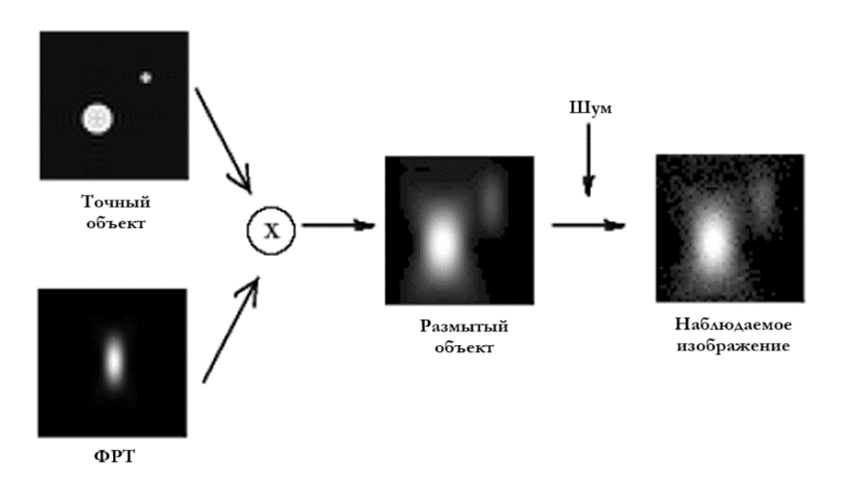
\includegraphics[keepaspectratio=true,scale=0.55] {my_folder/images/problem/start.png}
	\captionof{figure}{Схема свёртки точного объекта с ФРТ вместе с фотонным шумом}\label{fig:problem-start}  
	\vspace{\mfloatsep} % интервал  	
\end{minipage}
\par Не умоляя общности, рассмотрим изображения $I_x, I_y$, как дискретный набор значений. Тогда множества $\Omega_x, \Omega_y$ могут быть представлены, как пространства $\mathbb{R}^{l,r,c}$, где $l, r, c$ - число слоёв, высота и ширина каждого слоя изображения. В случае наличия нескольких каналов (например, $w$), пространства могуть быть представлены, как $\mathbb{R}^{l,r,c,w}$. Также важно отметить, что шум $N$ рассматривается, как элемент пространства $\mathbb{R}^{l,r,c} (\mathbb{R}^{l,r,c,w})$. Подробнее о природе шума и постановке задачи денойзинга будет рассмотрено в следующем пункте.
\par Методы восстановления "точного" изображения по наблюдаемому называются \textit{деконволюцией} (процесс обратный к свёртке). Общая задача восстановления изображения может быть сведена к выбору функции $\mathscr{F}(I_y)$:
\begin{equation}
	\hat{I_x} = \mathscr{F}(I_y)
\end{equation}
где $\hat{I_x}$ - аппрокимация $I_x, \hat{I_x} \in \Omega_x$
\par Однако зачастую процесс восстановления изображений рассматривается как два последовательных этапа: денойзинг (обесшумливание) изображений и сама деконволюция (т.е. процесс улучшения качества размытого снимка некоторого образца). Это обусловлено тем, что методы деконволюции искажают снимки при наличии шума.

\subsection{Постановка задачи денойзинга}
\par Флуоресцентная микроскопия характеризуется пуассоновско-гауссовым шумом (mixed Poisson–Gaussian, MPG), где пуассоновский шум является доминирующим источником шума.[2] Это объясняется тем, что количество фотонов, захваченных микроскопом, черезвычайно мало. Следовательно, измеренный оптический сигнал во флуоресцентной микроскопии квантуется из-за дискретной природы фотонов, и в изображениях, полученных с помощью флуоресцентной микроскопии, преобладает пуассоновский шум, а не гауссовский шум, который характерен для фотографии[*]. 
\par Шум может существенно ухудшать качество изображений и затруднять дальнейший анализ. Поэтому важно разработать алгоритм денойзинга, который будет эффективно удалять шум, сохраняя при этом важные структурные детали образцов.
\par Введём формальные обозначения для постановки задачи. Пусть $I_z = I_x * H$ - размытое изображение (свёртка точного объекта и ФРТ), не содержащая шумов. $I_z \in \Omega_z, \Omega_z \in \mathbb{R}^{l,r,c} (\mathbb{R}^{l,r,c,w})$ - множество размытых изображений объектов. Тогда задача денойзинга сводится к нахождению такой функции $\mathscr{F}_1(I_y)$, что:
\begin{equation}
	\hat{I_z} = \mathscr{F}_1(I_y)
\end{equation}
где $\hat{I_z}$ - аппрокимация $I_z, \hat{I_x} \in \Omega_x$.\\
Задача деконволюции сводится к поиску функции $\mathscr{F}_2(I_z)$: 
\begin{equation}
	\hat{I_x} = \mathscr{F}_2(I_z)
\end{equation}
где $\hat{I_x}$ - аппрокимация $I_x, \hat{I_x} \in \Omega_x$.\\
Общая задача восстановления изображений выглядит следующим образом:
\begin{equation}
	\hat{I_x} = \mathscr{F}_2(\mathscr{F}_1(I_y))
\end{equation}

Задача денойзинга трёхмерных изображений формулируется следующим образом:
\begin{itemize}[]
	\item Разработать алгоритм денойзинга трёхмерных изображений, где на вход поступает шумное изображение $I_y \in \mathbb{R}^{l,r,c}$, а на выходе получаем результат денойзинга: $I_z \in \mathbb{R}^{l,r,c}$ (см. \firef{fig:denoise-problem}).
	\item Исследовать природу шума на реальных снимках с конфокальных микроскопов и доказать эксперементальным способом, что он распределяется в большей мере по Пуассону с некоторым параметром $\lambda$:
	\begin{equation}
		P(\lambda) = \frac{\lambda^k e^{-\lambda}}{k!}
	\end{equation}
	где $\lambda$ - частота возникновения, уровень шума, $k$ - наблюдаемое значение случайной величины.
	
\end{itemize}
\begin{minipage}{\textwidth}
	\centering
	\vspace{\mfloatsep} % интервал  	
	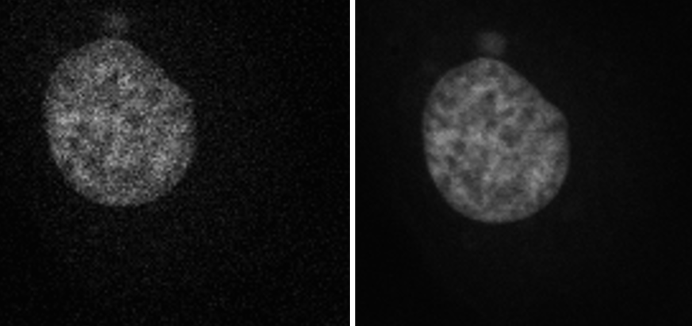
\includegraphics[keepaspectratio=true,scale=0.45] {my_folder/images/problem/denoisiong_example.png}
	\captionof{figure}{Пример работы денойзинга: слева - шумное изображение клетки, справа - обесшумленное (результат денойзинга)}\label{fig:denoise-problem} 
	\vspace{\mfloatsep} % интервал  	
\end{minipage}

\subsection{Постановка задачи автоматической сегментации сфер}
\par Для восстановления исходного изображения с помощью итерационных методов деконволюции необходимо в явном виде нахождение ФРТ. На практике точное значение ядра свёртки $H$ найти очень сложно, поэтому используют приближенное значение. Методы, создающие такие приближения, делятся на две группы: теоретические и экспериментальные.

\par Теоретические методы вычисляют ФРТ на основе определенных моделей и функций, тогда как экспериментальные методы включают съемку объектов очень малого размера, например, калибровочных флуоресцентных сфер. Функции рассеяния точки, полученные теоретическим путем, называют теоретическими ФРТ (тФРТ), а функции, полученные экспериментальным путем, — экспериментальными ФРТ (эФРТ). Оба метода обладают своими преимуществами и недостатками: так, например, теоретическая ФРТ не содержит шумов, которые могли бы приводить к неточностям при деконволюции, однако она же не отражает неточностей системы регистрации. Эксперементальный способ вычисления ФРТ имеет абсолютно обратные свойства.

\par Построение эФРТ происходит путём деконволюции размытой сферы, полученной из усреднения множества исходных, наблюдаемых с микроскопа снимков сфер, точным моделируемым изображением сферы. Более наглядное описание см на \firef{fig:autosegm-problem}. Стоит отметить тот факт, что чем больше размытых микроскопом снимков сфер участвует в усреднении, тем точнее получается эФРТ и, как следствие, результаты  аналитической деконволюции. Однако при извлечении большого количества сфер (80-100 и более), процесс сегментации может занять около 10-15 минут. Поэтому необходим автоматический подход, использующий методы компьютерного зрения, который позволил бы ускорить данный процесс, а также оставил возможность ручной корректировки результатов.
\begin{minipage}{\textwidth}
	\centering
	\vspace{\mfloatsep} % интервал  	
	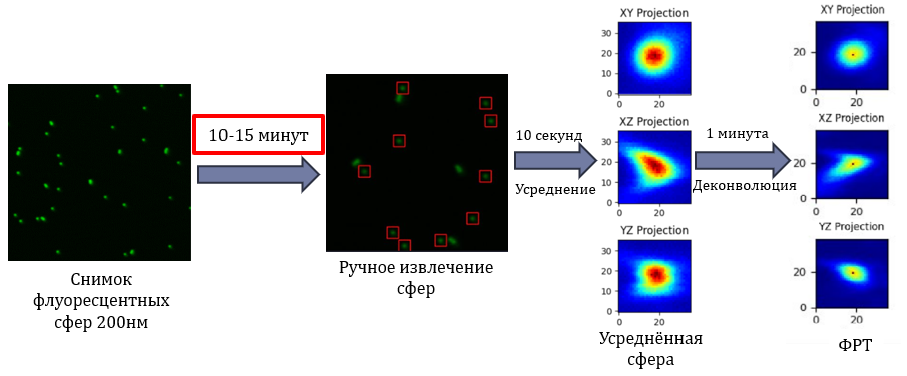
\includegraphics[keepaspectratio=true,scale=0.85] {my_folder/images/problem/segment_spheres.png}
	\captionof{figure}{Схема эксперементального способа вычисления ФРТ}\label{fig:autosegm-problem}  
	\vspace{\mfloatsep} % интервал  	
\end{minipage}

\section{Обзор литературы} \label{ch1:sec2}
\par В данном параграфе рассмотрено 2 ключевых подхода, которые будут использоваться для описания существующих методов, так и создания новых в следующей главе.
\subsection{Существующие методы деконволюции} 
\par \textit{Деконволюция} - это процесс восстановления оригинального изображения, которое было искажено в процессе съёмки. Глобально эти методы можно разбить на 2 группы: использующие функцию рассеяния точки ($H$) в процессе обработки, и не использующие. Вторую группу называют \textit{методами "слепой" деконволюции}, обычно дают менее точные результаты, если сравнивать с первой группой.
\par Рассмотрим подкласс алгоритмов первой группы, основанных на природе шума, которые называются \textit{статистические алгоритмы деконволюции}. Данный подкласс получен из алгоритма оценки максимального правдоподобия (MLE), написанного для минимизации пуассоновского шума на изображении[*]. 

\par \textit{Метод Ричардсона-Люси (RL)} основан на методе максимального правдоподобия и предназначен для работы с шумами, следующими закону распределения Пуассона. Этот алгоритм итеративно улучшает оценку объекта, исходя из текущей оценки, наблюдаемого изображения и известной ФРТ.
\begin{equation}
	\hat I^{k+1}_x = I^{k}_x(\frac{I_z}{I^{k}_x\circledast H})\circledast H^*
\end{equation}
где $I^k_x$ - текущее приближение на итерации k, $I_z$ - наблюдаемое (размытое) изображение, $H$ – функция рассеяния точки, $H^*$ - обратное ядро свёртки (ФРТ, повёрнутая относительно начала координат на 180 градусов).
\par Этот алгоритм обладает свойством неотрицательности, т.е. если начальное значение неотрицательно, то и все последующие итерации будут неотрицательными. Однако, при наличии шума алгоритм может сходиться к решению, доминируемому шумом, что ухудшает качество изображения. Помимо использования методов денойзинга для решения проблемы усиления шума, существуют модификации RL-алгоритма с добавлением регуляризационных членов. Разберём наиболее часто используемые модификации:
\begin{enumerate}[]
	\item \textit{Регуляризация Тихонова-Миллера (TM)}:\\
	\begin{equation}
		\hat I^{k+1}_x = I^{k}_x(\frac{I_z}{I^{k}_x\circledast H}\circledast H^*)\cdot(1 - 2\lambda_{TM}\nabla^2 I^{k}_x)
	\end{equation}
	где $\lambda_{TV}$ - параметр регуляризации, а $\nabla^2$ - лапласиан объекта.
	\item Общая вариация(Total variation, TV):\\
	TV-регуляризация сохраняет контуры и границы объектов, уменьшая шум в однородных областях.
	\begin{equation}
		TV(I_x) = \int |\nabla I_x| \, dxdydz
	\end{equation}
	\begin{equation}
		\hat I^{k+1}_x = I^{k}_x(\frac{I_z}{I^{k}_x\circledast H}\circledast H^*) - \lambda_{TV}\cdot TV(I^{k}_x)
	\end{equation}
	где $\lambda_{TV}$ - параметр регуляризации.
\end{enumerate}

\subsection{Элементы свёрточных нейронных сетей}
\par В данном подпараграфе будет представлен краткий обзор архитектурных элементов свёрточных нейронных сетей (CNN), которые играют ключевую роль в обработке и анализе изображений. 

\subsubsection{Свёрточный слой}
\par \textit{Свёрточный слой (Convolutional Layer)} является ключевым элементом CNN, часто используется для обработки изображений. Этот слой выполняет операцию свёртки (convolution), которая позволяет извлекать различные признаки из входных данных.
\par Операция свёртки двух функций $f$ и $g$ записывается так:
\begin{equation}
	(f*g)(x) = \int_{\mathbb{R^n}}^{} f(y)g(x-y)\,dy
\end{equation}
где $f,g: \mathbb{R^n} \Rightarrow \mathbb{R}$ - интегрируемые функции по мере Лебега на $\mathbb{R}^n$, а $(f*g)(x): \mathbb{R^n} \Rightarrow \mathbb{R}$.
Назовём $f(x)$ вход, $g(x)$ - ядро, а результат $(f*g)(x)$ - карта признаков.
\par Распишем понятния в рамках нашей задчи:\\
\textit{Фильтр(ядро свёртки)} – это матрица небольшого размера, которая скользит по изображению и выполняет операцию свёртки. Пусть задана размером $k \times k$.
\textit{Свёртка} - это операция, при которой фильтр скользит по входному изображению и вычисляет сумму произведений элементов фильтра и соответствующих элементов области изображения. Если входное изображение имеет размер $r \times c$ и фильтр $k \times k$, то выходное будет иметь размер $(r-k+1) \times (c-k+1)$ без применения дополнения (\textit{padding}). Если у нас n фильтров, то рамзер будет: $(r-k+1) \times (c-k+1) \times n$.
\par Свёрточные слои могут иметь несколько каналов. В этом случае, каждый канал имеет свой собственный фильтр, и результаты свёртки с каждым каналом суммируются.
\par Рассмотрим формулу свёрточного слоя двухмерного изображения с одним фильтром и одним каналом изображения.
\begin{equation}
	O(i,j) = (I*K)(i,j) = \sum_{u=0}^{k-1}\sum_{v=0}^{k-1}I(i+u, j+v) \cdot K(u,v)
\end{equation}
где $I$ - входное изображение размером $r \times c$, $K$ -фильтр размером $k \times k$, $O$ - выходное изображение, результат свёртки, $i=0,1,.., r-k$ и $j=0,1,.., c-k$ - точки карты признаков.
\par Также рассмотрим применения "дополнения" (Padding) и "шага" (Stride) для свёрточных слоёв:
\begin{enumerate}[]
	\item Padding добавляет рамку из нулей вокруг входного изображения, чтобы контролировать размер выходного изображения. Например, чтобы сохранить размер выходного изображения, если применить $p = \frac{k-1}{2}$, для фильтра размером $k \times k$
	\item Stride – это шаг, с которым фильтр скользит по изображению. Если шаг равен 
	$s$, то выходное изображение будет иметь размер:
	\begin{equation}
		(\frac{r-k}{s}) + 1 \times (\frac{c-k}{s}) + 1 
	\end{equation}
\end{enumerate}

\subsubsection{Слой объединения (Pooling-слой)}
\par \textit{Слой объединения (Pooling Layer)} используется для уменьшения пространственных размеров карт признаков и количества параметров, сохраняя при этом наиболее важную информацию. 
\par Наиболее распространённые слои объединения:
\begin{itemize}[]
	\item Максимальное объединение (Max Pooling). Этот метод выбирает максимальное значение из квадратной области во входной карте признаков. 
	\item Усреднение (Average Pooling). Этот метод вычисляет среднее арифмитическое значение в каждой квадратной области входной карты признаков.
\end{itemize}
\par Pooling-слои помогают уменьшить количество параметров в модели и контролировать переобучение.

\subsubsection{Слой повышения дискретизации (UpSampling-слой)}
\par \textit{Слой повышения дискретизации (UpSampling Layer)} выполняет обратную функцию Pooling-слоя. Его основная задача состоит в увеличении разрешения входных данных, поэтому он не содержит весов. Данный слой особенно полезен в задачах сегментации изображений и генеративных моделях. 
\par Основные методы повышения дискретизации:
\begin{itemize}[]
	\item Билинейная интерполяция (Bilinear Interpolation). Этот метод использует линейную интерполяцию между ближайшими пикселями для заполнения новых пикселей в увеличенном изображении. 
	\item Максимальное объединение (Max Unpooling). Этот метод сохраняет максимальные значения из предыдущего слоя объединения и заполняет ими новые увеличенные области.
	\item Транспонированная свертка (Transpose Convolution). Этот метод применяет операцию, обратную свертке. В отличие от обычной свертки, транспонированная свертка увеличивает пространственные размеры входных данных, заполняя новые значениями, вычисляемыми на основе весов фильтра. 
\end{itemize} 

\subsubsection{Слой активации}
Слой активации (Activation Layer) вводит нелинейность в модель, что позволяет сети обучаться сложным функциям отображения. 
Наиболее распространённые функции активации:
\begin{itemize}[]
	\item \textit{Сигмоидальная функция (Sigmoid)}:\\
	Она преобразует входные значения в диапазон от 0 до 1. Недостаток этой функции – проблема исчезающего градиента(vanishing gradient problem) при обратном распространении ошибки.
	\begin{equation}
		\sigma(x) = \frac{1}{1+e^{-x}}
	\end{equation}
	\item \textit{ReLU (Rectified Linear Unit)}:\\
	Эта функция обнуляет отрицательные значения и сохраняет положительные без изменений. Она решает проблему затухания градиента, но имеет свои минусы: некоторые нейроны могут "умирать", становясь неактивными на протяжении всего обучения. Также ReLU несимметрична относительно нуля, что может привести к проблеме "расслоения", когда нейроны выдают только положительные значения.
	\begin{equation}
		ReLU(x) = \max(0, x)
	\end{equation}
	\item \textit{Leaky ReLU}:\\
	В отличие от ReLU, Leaky ReLU возвращает само значение при положительном входе, а при отрицательном – линейную функцию от входа, умноженную на небольшой коэффициент, называемый "утечкой" (leak). Это предотвращает "умирание" нейронов и способствует лучшей сходимости и более точному обучению сети.
	\begin{equation}
		Laeky ReLU(x) = \max(\alpha\cdot x, x)
	\end{equation}
	\item \textit{Гиперболический тангенс (Tanh)}:\\
	Эта функция преобразует входные значения в диапазон от -1 до 1. Она также помогает уменьшить проблему исчезающего градиента и имеет более пологую кривую по сравнению с сигмоидальной функцией, что позволяет сети лучше распознавать сложные зависимости в данных. Гиперболический тангенс также имеет гладкую производную, что полезно для алгоритмов оптимизации, требующих вычисления градиента.
	\begin{equation}
		\tanh(x) = \frac{e^x-e^{-x}}{e^x+e^{-x}}
	\end{equation}
\end{itemize}

\subsubsection{Слой пакетной нормализации}
\par \textit{Слой пакетной нормализации (Batch Normalization Layer)} - это метод нормализации промежуточных слоёв нейронной сети для ускорения и стабилизации процесса обучения. Этот метод помогает справляться с проблемами, такими как затухание или взрыв градиентов, и улучшает общую производительность сети.
\par Пакетная нормализация решает проблему так называемого "внутреннего ковариационного сдвига" (internal covariate shift), который возникает, когда распределение активаций каждого слоя меняется в процессе обучения. Это может замедлять обучение, так как каждый слой сети должен адаптироваться к изменяющемуся распределению входов.



%% Вспомогательные команды - Additional commands
%
%\newpage % принудительное начало с новой страницы, использовать только в конце раздела
%\clearpage % осуществляется пакетом <<placeins>> в пределах секций
%\newpage\leavevmode\thispagestyle{empty}\newpage % 100 % начало новой страницы	         	 % Глава 1
\ContinueChapterBegin % размещать главы <<подряд>> 
\chapter{Описание методов} \label{ch2}
Данная глава посвящена методам и алгоритмам, используемых в исследовании для обработки и анализа трёхмерных изображений. Глава включает в себя описание разработанных алгоритмов 3D денойзинга и автоматической сегментации флуоресцентных сфер, а также описание уже существующих подходов для предлагаемого решения. 
\section{Описание алгоритма 3D денойзинга} \label{ch2:sec1}
\par В этом параграфе подробно рассмотрены методы шумоподавления двумерных снимков, такие как Non-local Means и Noise2Noise, а также предлагаемое решение в виде комбинации этих методов и их модификации, способное эффективно устранять шум на трёхмерных изображениях с микроскопа.
\subsection{Описание алгоритма NLM (Non-local means)}	
\par Классически существуют два типа моделей по шумоподавлению, а именно локальные и нелокальные. Преимущество первого подхода заключается в его скорости, однако его недостаток состоит в невозможности эффективного сохранения краёв изображений, что проявляется в виде размытия границ и деталей на изображении. Примером локального подхода является Гауссово размытие, а нелокального - метод Non-local means(NLM)\cite{nlm2011}.
%\subsubsection{Размытие по Гауссу}
%\subsubsection{Non-local means}
\par NLM (Non-local means) - это алгоритм для устранения шума на изображении, который обновляет значения пикселей на основе взвешенного среднего значений других пикселей, определённых как наиболее схожие. В отличие от локальных методов, которые используют значения соседних пикселей, NLM использует информацию из всего изображения, что позволяет ему лучше сохранять детали и текстуры. Диаграмма деятельности метода Non-local means приведена ниже на \firef{fig:nlm-schema}.
\par \textbf{Алгоритм метода нелокального среднего (NLM)}\cite{nlm2015}
\begin{enumerate}[]
	\item \textit{Создание окна поиска}:\\
	Создаётся большое окно поиска $S$ размером $K \times K$, центрированное на пикселе $p$. Одновременно создаётся патч(блок пикселей) $N_p$ размером $L$, центрированный на пикселе $p$.
	\item \textit{Вычисление схожести патчей}:\\
	В окне поиска устанавливается новый патч $N_q$, центрированный на пикселе $q$. Затем вычисляется евклидово расстояние $d(p,q)$ между $N_p$ и $N_q$. Далее производится взвешивание патчей с использованием гауссовой функции:
	\begin{equation}
		\tilde w(p,q) = e^{-\frac{d(p,q)}{h^2}}
	\end{equation}
	где $h$ - параметр фильтрации (сглаживания),\\
	$d(p,q) = \|I_y(N_p) - I_y(N_q)\|^2_2$ - евклидово расстояние между $N_p, N_q$\\
	Для наглядности приведен \firef{fig:nlm-weights}, на котором представлена концепция схожести патчей:\\
	\begin{minipage}{\textwidth}
		\centering
		\vspace{\mfloatsep} % интервал  	
		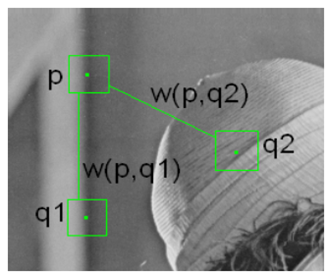
\includegraphics[keepaspectratio=true,scale=0.47] {my_folder/images/denoising/nlm_weights.png}
		\captionof{figure}{Пример,иллюстрирующий концепцию схожестей\\патчей с 3 пикселями: $p, q_1, q_2$ и их весами:\\$w(p, q_1), w(p, q_2)$. $w(p, q_1) > w(p, q_2)$,\\ т.к. патч с $p$ более похож на пачт с $q_1$, чем с $q_2$ }\label{fig:nlm-weights}
		\vspace{\mfloatsep} % интервал  	
	\end{minipage}
	\item \textit{Нормализация весов}:\\
	Проход по всем точкам $q (N_q \in S)$ и нормализация весов:
	 \begin{equation}
		w(p,q) = \frac{\tilde w(p,q)}{\sum_{q \in S} \tilde w(p,q)} 
	\end{equation}
	Согласно формулам, коэффициент веса удовлетворяет условиям:
	\begin{equation}
		\left\{ 
		\begin{array}{ll} 
			\sum_{q} w(p,q) = 1\\
			0 \leq w(p,q) \leq 1 \end{array}\right.
	\end{equation}	
	\item \textit{Вычисление результирующего значения}:\\
	Вычисление результирующего значения обесшумленного пикселя с помощью взвешенной суммы:
	\begin{equation}
		I_z(p) = \sum_{q \in S}w(p,q)I_y(q)
	\end{equation}
\end{enumerate}

\begin{minipage}{\textwidth}
	\centering
	\vspace{\mfloatsep} % интервал  	
	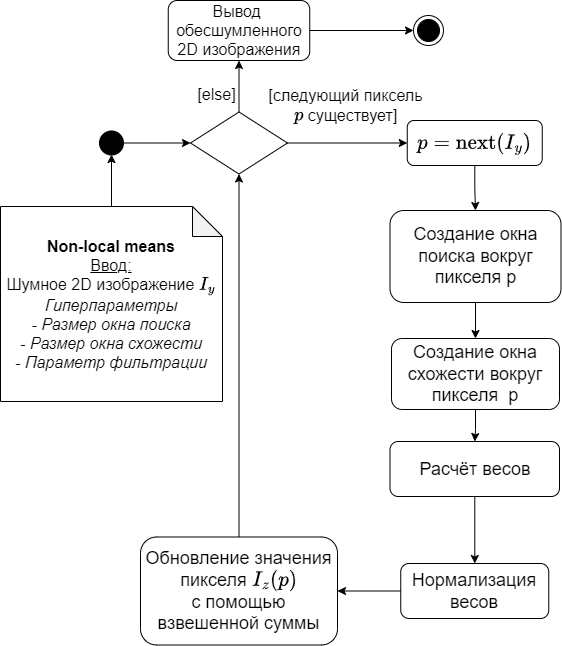
\includegraphics[keepaspectratio=true,scale=0.47] {my_folder/images/denoising/pipeline_nlm_ru.png}
	\captionof{figure}{Диаграмма деятельности Non-local means}\label{fig:nlm-schema}  
	\vspace{\mfloatsep} % интервал  	
\end{minipage}
\subsection{Описание модели Noise2Noise}
\par В качестве метода глубокого обучения была выбрана модель Noise2Noise \cite{noise2noise2018}. Данный подход часто применяется для обработки шумных изображений, таких как флуоресцентные микроскопические снимки с пуассоновско-гауссовым шумом (MPG). В данном описании рассматривается модифицированная версия модели Noise2Noise, включающая дополнительные слои активации, адаптивное обучение и настроенные гиперпараметры. 
\par \textbf{Архитектура сети} изображена на \firef{fig:noise2noise} и представляет собой свёрточную нейронную сеть (CNN), состоящую из энкодера (Encoder) и декодера (Decoder), разбитых на 5 уровней повышения/понижения дискретизации. Каждый уровень состоит из последовательно идущих 2D свёрточных слоёв 3x3, пакетной нормализации, слоя активации Leaky ReLU и соответствующего слоя повышения/понижения дискретизации \cite[с. 337-338]{denoising-imagej-22}. 
\par Из описания архитектуры можно заметить, что данная нейронная сеть является \textit{полносвёрточной}, так как состоит из слоёв свёртки, повышения и понижения дискретизации, активации и пакетной нормализации. Для данной задачи сеть обладает важным свойством - способность обрабатывать входные данные различных размеров. Для данной сети имеется 5 уровней понижения/повышения дискретизации, единственным ограничением на размер входных изображений будет кратность $2^5 = 32$ вдоль всех осей.
\begin{minipage}{\textwidth}
	\centering
	\vspace{\mfloatsep} % интервал  	
	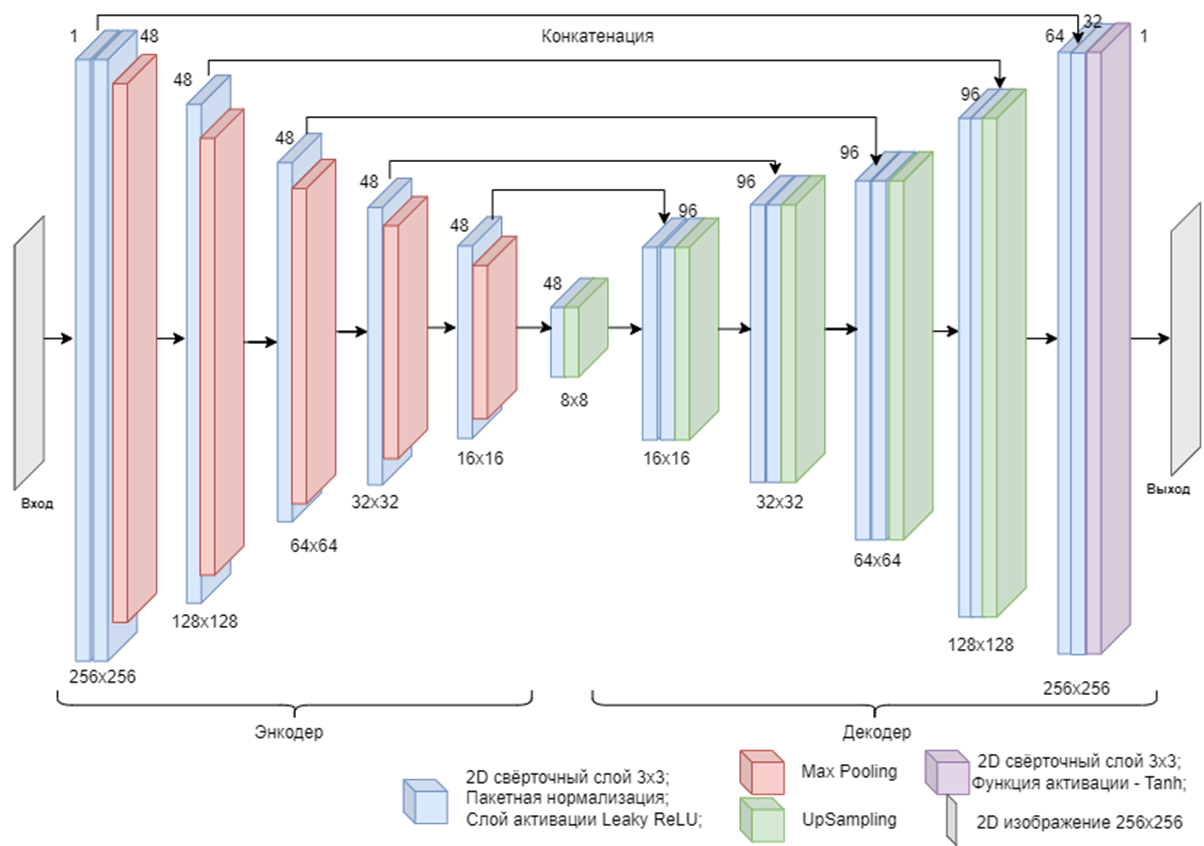
\includegraphics[keepaspectratio=true,scale=0.47] {my_folder/images/denoising/n2n_architecture.png}
	\captionof{figure}{Архитектура сети Noise2Noise}\label{fig:noise2noise}  
	\vspace{\mfloatsep} % интервал  	
\end{minipage}
\par \textbf{Основная идея} Noise2Noise заключается в том, что обучение происходит на паре зашумлённых изображений. Данный факт позволяет сети эффективно удалять шум без необходимости использования чистых изображений в процессе обучения:
\begin{itemize}[]
	\item Вместо использования чистого изображения в качестве цели (label), как это делается в традиционных методах, Noise2Noise использует другое зашумленное изображение того же объекта в качестве цели.
	\begin{equation}
		{I_y}_1 = I_z + N_1,\
		{I_y}_2 = I_z + N_2,\
		\hat I_z = \mathscr{F}_1({I_y}_1)
	\end{equation}
	где $I_z$ - точный сигнал, $N_1, N_2$ - разные шумы, порождающие разные входное и целевое изображения соответственно: ${I_y}_1, {I_y}_2$, $\hat I_z$ - восстановленное изображение, результат $\mathscr{F}_1$.\\
	Поскольку $N_1, N_2$ - случайные величины, они не коррелируют между собой, что позволяет модели учиться выделять общий сигнал $I_z$ присутствующий в обоих изображениях.
	\item Это позволяет модели учиться на данных, где шум разный (например, разные условия съёмки), но сам объект остается неизменным.
	\item Данное свойство делает его особенно полезным в реальных сценариях, где получение чистых данных затруднено или невозможно.
\end{itemize}
\par Данную задачу можно отнести к классу задач с семантическим
разрывом, следовательно, можно выделить класс функций $\mathscr{F}_1(I_y, \theta)$, который позволит найти искомую функцию $\mathscr{F}_1(I_y)$:
\begin{equation}
	\mathscr{F}_1(I_y) = \mathscr{F}_1(I_y, \hat \theta)
\end{equation} где параметр $\hat \theta$ ищется следующим образом:
\begin{equation}
	\hat\theta = \arg\min_{\theta}\mathscr{L}(\hat I_z, {I_y}_2) = \arg\min_{\theta}\mathscr{L}(\mathscr{F}_1(I_y), {I_y}_2)
\end{equation}
где $\theta$ - веса рассматриваемой модели, $\mathscr{L}$ - функция ошибки.\\
В качестве функции потерь $\mathscr{L}$ была взята среднеквадратичная ошибка (MSE), так как она хорошо штрафует за выбросы:\\
\begin{equation}
	MSE(\hat I_z, {I_y}_2) = \frac{1}{N}\sum_{i=1}^{N}(\hat {I_z}_i - {I_y}_{2,i})^2
\end{equation}
где $i = 1..N$ - параметр итерирования по всем точкам изображения, $N$ - общее число точек в изображении.
\par \textbf{Основные модификации модели Noise2Noise}
\begin{itemize}[]
	\item \textit{Нелинейный слой активации (tanh)}:\\
	В исходной архитектуре Noise2Noise используется линейный выходной слой. В модифицированной версии добавлен нелинейный слой активации (tanh) после финального свёрточного слоя. Это помогает лучше моделировать сложные зависимости и улучшает качество денойзинга.\\
	Гиперболический тангенс:
	\begin{equation}
		y_i = \frac{e^{x_i} - e^{-x_i}}{e^{x_i} + e^{-x_i}}
	\end{equation}
	преобразует входное значение в выходное в диапазоне $[-1, 1]$ на $i$-ом слое.
	\item \textit{Адаптивное обучение}:\\ 
	Для ускорения и улучшения процесса обучения используется стратегия адаптивного обучения, известная как \textit{one cycle policy}. Используется линейно-косинусное изменение скорости обучения - сначала происходит линейное увеличение скорости обучения, а затем её косинусное уменьшение.
	\begin{equation}
		\left\{ \begin{aligned} 
			lr(t)= lr_{low} + \frac{t}{start} \times (lr_{max} - lr_{low}), t \leq t_{start},\\
			lr(t)= lr_{end} + \frac{lr_{max} - lr_{end}}{2} \times (\cos(\pi\times t) + 1), t > t_{start}\ldots
		\end{aligned} \right.
	\end{equation}
	$t \in [0, 1]$ - процент выполнения обучения\\
	$t_{start} = 0.3$ - момент перехода от линейного к косинусному изменению\\
	$lr_{max} = 0.0001$ - максимальная скорость обучения\\
	$lr_{low} = \frac{lr_{max}}{25}$ - стартовая скорость обучения, $div = 25$\\
	$lr_{end} = \frac{lr_{max}}{10^4}$ - минимальная скорость обучения\\
\end{itemize}

\subsection{Описание предлагаемого решения}
\par Помимо реализованных алгоритмов денойзинга двухмерных изображений, описанных выше, был разработан алгоритм шумоподавления трёхмерных снимков, комбинирующий в себе оба метода, позволяющий совмещать некоторые достоинства каждого из них.
\par Общая структура предлагаемого алгоритма представлена на \firef{fig:3d-denoise-schema}. Процесс обработки трёхмерных изображений делится на три этапа:
\begin{enumerate}[]
	\item \textit{Предварительная обработка трёхмерного изображения}, включающая следующие шаги:\\
	\begin{enumerate}[]
		\item Перевод изображения в монохром
		\item Z-нормализация
		\begin{equation}
			x_{normalized} = \frac{x-\mu}{\sigma}
		\end{equation}
		где $\mu$ - среднее, $\sigma$ - СКО конкретного слоя
		\item MinMax нормализация
		\begin{equation}
			x_{scaled} = \frac{x - x_{min}}{x - x_{max}}
		\end{equation}
		где $x_{\min}, x_{\max}$ - минимальные максимальные значения всего трёхмерного изображения
	\end{enumerate}
	\item \textit{Основной этап обработки изображения}.\\ Результат предобработки передаётся на вход основному этапу, где пользователь задаёт способ обработки изображений: нелокальный фильтр, нейросетевой подход или их комбинации в различном порядке. Денойзинг производится для каждого слоя независимо друг от друга.
	\item \textit{Склейка слоёв}.\\ На выход подаётся трёхмерное изображение, склеенное из обработанных ранее слоёв.
\end{enumerate}
%\subsubsection{Алгоритм денойзинга трёхмерных снимков}
\begin{minipage}{\textwidth}
	\centering
	\vspace{\mfloatsep} % интервал  	
	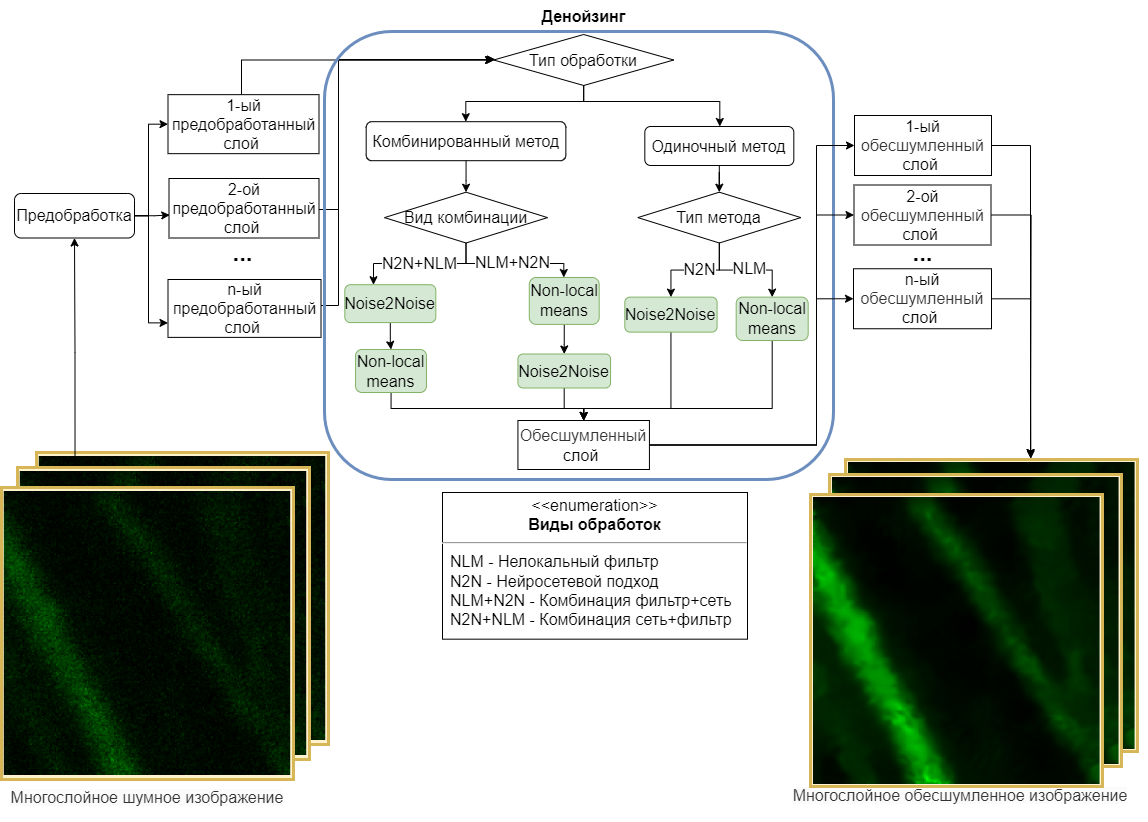
\includegraphics[keepaspectratio=true,scale=0.3] {my_folder/images/denoising/schema_denoising.png}
	\captionof{figure}{Алгоритм 3D денойзинга}\label{fig:3d-denoise-schema}  
	\vspace{\mfloatsep} % интервал  	
\end{minipage}

\section{Описание алгоритма автоматической сегментации флуоресцентных сфер} \label{c2:sec2}
\par Для ускорения процесса ручной сегментации был предложен автоматический подход с использованием методов компьютерного зрения. Для наглядности работы алгоритма продемонстрирована диаграмма деятельности на \firef{fig:autosegm-schema}.
\par \textbf{Алгоритм автоматической сегментации сфер}
\begin{enumerate}
	\item Проведение предварительной обработки
	\begin{enumerate}[]
		\item Перевод изображения в монохром
		\item Применение Гауссова размытия с использованием гиперпараметра радиуса размытия
		\begin{equation}
			G(x,y) = \frac{1}{2\pi\sigma^2}e^{-\frac{x^2+y^2}{2\sigma^2}}
		\end{equation}
		где $x, y$ - координаты точки, $\sigma$ - радиус размытия (стандартное отклонение Гауссового распределения).\\
		Изображение сворачивается с Гауссовым ядром -  каждый пиксель изображения заменяется взвешенной суммой соседних пикселей, где веса определяются значениями Гауссового ядра.
		\item Бинаризация с гиперпараметром порога бинаризации
	\end{enumerate}
	\item Анализ связанных компонент \cite[с. 679-682]{connected-components-2008} - этап, на котором происходит детекция всех сфер (и слипшихся, и одиночных; пример видов сфер на \firef{fig:sphere-types}). Результат анализа - вывод следующих параметров: количество компонент связанности (количество сфер), статистика компонент (координаты границ сфер, объёмы сфер), центроиды (центры сфер).
	\begin{figure}[H]
		\adjustbox{minipage=0.5em,valign=t}{\subcaption{}\label{fig:train-iters-a}}%
		\begin{subfigure}[t]{\dimexpr.5\linewidth-0.5em\relax}
			\centering
			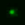
\includegraphics[width=.2\linewidth,valign=t]{my_folder/images/autosegm/good_bead.png}
		\end{subfigure}
		\hfill %выровнять по ширине
		\adjustbox{minipage=0.5em,valign=t}{\subcaption{}\label{fig:train-iters-b}}%
		\begin{subfigure}[t]{\dimexpr.5\linewidth-0.5em\relax}
			\centering
			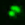
\includegraphics[width=.2\linewidth,valign=t]{my_folder/images/autosegm/bad_bead.png}
		\end{subfigure}
		\\[20pt]
		\captionsetup{justification=centering} %центрировать
		\caption{Виды сфер в результате анализа связанных компонент: {\itshape a} --- одиночная сфера; {\itshape b} --- слипшиеся сферы} 
		\label{fig:sphere-types}
	\end{figure}
	\item Фильтрация сфер на основе предложенного объёма правильной (одиночной) сферы. Если объём конкретной сферы меньше заданного, то она распознаётся как правильная и сохраняется.
	\item Извлечение трёхмерных сфер с заданным гиперпараметром ограничивающего прямоугольника.
	\item Усреднение флуоресцентных сфер. Считается выборочное среднее по всем извлечённым.  
	\item Вывод результатов (усреднённой сферы и снимка с сегментированными сферами).
\end{enumerate}
\begin{minipage}{\textwidth}
	\centering
	\vspace{\mfloatsep} % интервал  	
	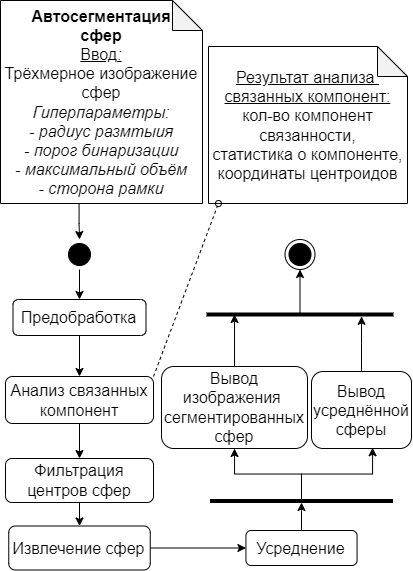
\includegraphics[keepaspectratio=true,scale=0.4] {my_folder/images/autosegm/schema.png}
	\captionof{figure}{Диагрпамма деятельности автоматической сегментации сфер}\label{fig:autosegm-schema}  
	\vspace{\mfloatsep} % интервал  	
\end{minipage}
\textbf{Замечание}
\par Значения гиперпараметров подбирались экспериментальным  способом. Благодаря быстрой работе методов и заданным значениям по умолчанию, у человека есть возможность менять показатели в реальном времени, отслеживая динамику работы.
	         	 % Глава 2
\chapter{Результаты} \label{ch3}
\par Данная глава посвящена анализу результатов экспериментов по денойзингу с использованием различных методов, а также автоматической сегментации трёхмерных сфер. Особое внимание уделяется результатам интеграции и внедрения реализованных методов в онлайн-сервис.
\section{Результаты денойзинга}
\par В этом разделе особое внимание уделяется процессу обучения модели Noise2Noise, а также экспериментам, проводившимся на реальных и синтетических снимках различными методами денойзинга.
\subsection{Используемые метрики}
\par Для оценки качества работы методов денойзинга использовались следующие метрики \cite[с. 6-8]{zhang2019poissongaussian}:
\begin{enumerate}
	\item Время работы - время, затраченное на выполнение процесса денойзинга.
	\item Корень из средней квадратичной ошибки(RMSE)\\
	Среднеквадратичная ошибка(СКО):
	\begin{equation}
		MSE(I_1, I_2) = \frac{1}{N} \sum_{i,j,k}^{}(I_{1(i,j,k)} - I_{2(i,j,k)})^2
	\end{equation}
	Доля ошибки RMSE: 
	\begin{equation}
		RMSE(I_1, I_2) = \sqrt{\frac{MSE(I_1, I_2)}{N}}
	\end{equation}
	где $I_1, I_2$ - изображения одинаковой размерности, $i, j, k$ - переменные итерирования по всем точкам слоя изображения, $N = l \cdot r \cdot c$ - число всех точек в изображениях, $l$ - число слоёв изображений, $r$ - высота каждого слоя, $c$ - ширина каждого слоя.
	\item Отношение пикового сигнала к шуму (PSNR) 
	\begin{equation}
		PSNR(I_1, I_2) = 10\log_{10} \Big(\frac{R^2}{MSE}\Big)
	\end{equation}
	где $R$ - максимальное возможное значение пикселя в изображении.\\
	Если значения в каждой точке изображения кодируются, например, тремя цветами, каждый из которых хранится в 8 битах, то максимальное значение R будет следующим:
	\begin{equation}
		R = 2^8 = 256
	\end{equation}
\end{enumerate}

\subsection{Результаты тренировки нейронной сети Noise2Noise}
\par В данной задаче использовался метод обучения с учителем (supervised learning) для оценки параметров шума Пуассона на изображениях. В качестве минимизируемой функции применялась метрика MSE. Обучение осуществлялось с использованием нейронной сети Noise2Noise, которая позволяла эффективно обучаться без необходимости иметь точное изображение в паре. 
\par Для обучения использовался FMD (Fluorescence Microscopy
Denoising) датасет \cite[с. 4-6]{zhang2019poissongaussian}, состоящий из 12 000 изображений с различным уровнем шума [1, 2, 4, 8, 16] (итого 60 000 изображений). Тренировочный набор данных был разделён на 2 выборки: тренировочную и валидационную в отношении 4:1.
\par Процесс обучения был сопровождён следующими параметрами:
\begin{itemize}[]
	\item Оптимизатор Адама (Adam - Adaptive Moment Estimation)\cite[с. 4-10]{adam2022}, выбранный за его эффективность и способность адаптивно изменять скорость обучения.
	\item Размер batch = 10, что позволило эффективно использовать память GPU и стабилизировать процесс обучения.
	\item Установлена скорость обучения на 0.0001 с последующим применением линейно-косинусной функции изменения.
	\item Число эпох: 250, что оказалось оптимальным для предотвращения переобучения.
\end{itemize}
\par Обучение проводилось на вычислительном кластере из 4 GPU V100 64Гб, предоставленном Yandex DataSphere. Процесс занял около 45 минут, включая загрузку данных, обучение модели и оценку результатов на валидационных данных. 

\par Каждые 5 эпох проводился тест на различных изображениях. Это позволяло отслеживать динамику обучения. Выводился визуальный анализ из 8 разных изображений \firef{fig:train-iters}.

\begin{figure}[H]
	\adjustbox{minipage=1.3em,valign=t}{\subcaption{}\label{fig:train-iters-a}}%
	\begin{subfigure}[t]{\dimexpr.5\linewidth-1.3em\relax}
		\centering
		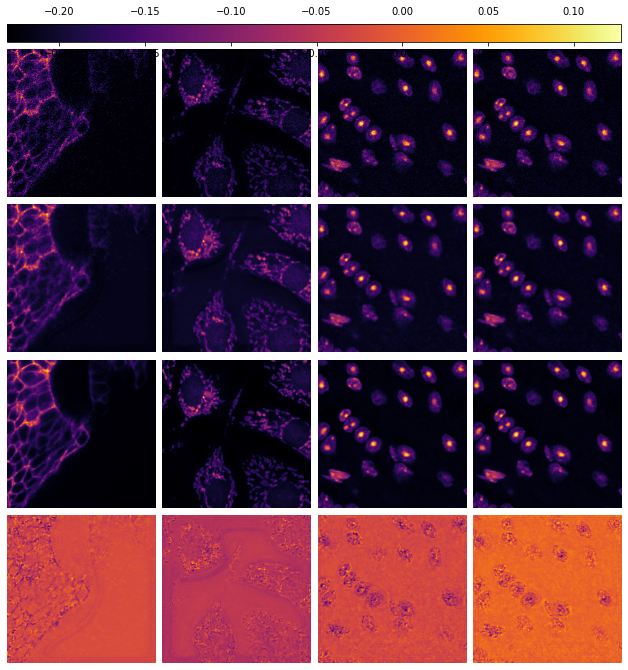
\includegraphics[width=.65\linewidth,valign=t]{my_folder/images/denoising/fix_test_epoch_50.png}
	\end{subfigure}
	\hfill %выровнять по ширине
	\adjustbox{minipage=1.3em,valign=t}{\subcaption{}\label{fig:train-iters-b}}%
	\begin{subfigure}[t]{\dimexpr.5\linewidth-1.3em\relax}
		\centering
		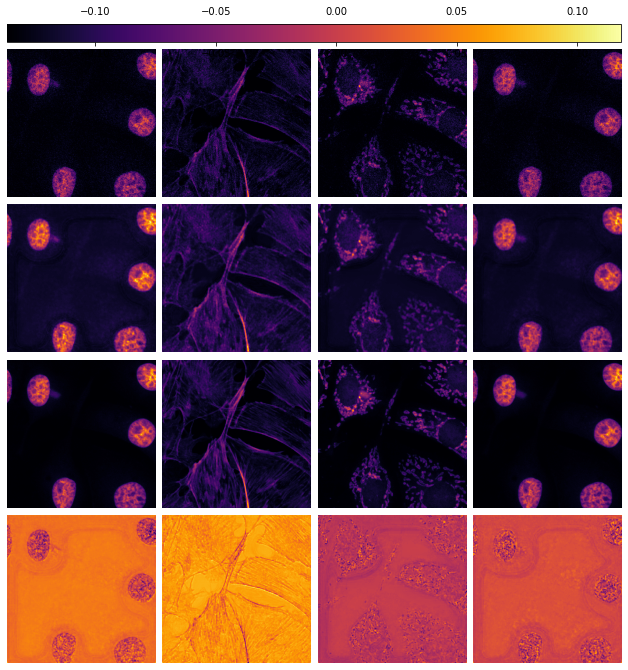
\includegraphics[width=.65\linewidth,valign=t]{my_folder/images/denoising/fix_test2_epoch_50.png}
	\end{subfigure}
	\\[20pt]
	\captionsetup{justification=centering} %центрировать
	\caption{Визуальный анализ на 50 эпохе, содержащий несколько тестовых изображений (слева-направо), а также этапы денойзинга (сверху-вниз): чистое изображение, зашумлённое, обесшумленное, разница между обесшумленным и чистым: {\itshape a} --- тест из 1-ых 4-ёх изображений; {\itshape b} --- тест из 2-ых 4-ёх изображений} 
	\label{fig:train-iters}
\end{figure}

\textbf{Итоговые результаты}.
В конце обучения были построены графики сходимости метрики PSNR и RMSE. Оценки показали высокую точность предсказаний \firef{fig:denoising-training-metrics}.

\begin{figure}[H]
	\adjustbox{minipage=1.3em,valign=t}{\subcaption{}\label{fig:denoise-train-a}}%
	\begin{subfigure}[t]{\dimexpr.5\linewidth-1.3em\relax}
		\centering
		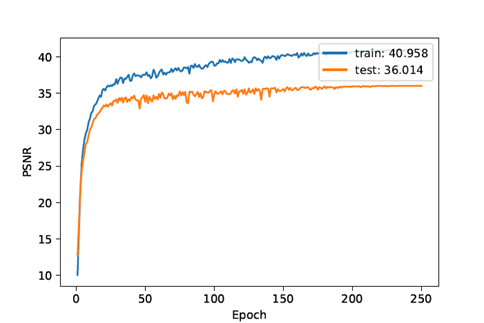
\includegraphics[width=.95\linewidth,valign=t]{my_folder/images/denoising/psnr_training.png}
	\end{subfigure}
	\hfill %выровнять по ширине
	\adjustbox{minipage=1.3em,valign=t}{\subcaption{}\label{fig:denoise-train-b}}%
	\begin{subfigure}[t]{\dimexpr.5\linewidth-1.3em\relax}
		\centering
		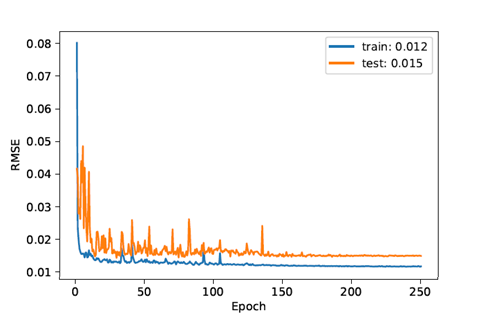
\includegraphics[width=.95\linewidth,valign=t]{my_folder/images/denoising/rmse_training.png}
	\end{subfigure}
	\\[20pt]
	\captionsetup{justification=centering} %центрировать
	\caption{Графики, отображающие метрии PSNR и RMSE в процессе обучения на протяжении всех 200 эпох. Синий график - результаты на тренировочной выборке; оранжевый - результаты на валидационной выборке: {\itshape a} --- метрика PSNR; {\itshape b} --- метрика RMSE} 
	\label{fig:denoising-training-metrics}
\end{figure}

\subsection{Эксперементы денойзинга}
\par В этом подпараграфе будет рассмотрен подробный анализ работы алгоритма 3D денойзинга с использованием различных методов, как нейросети Noise2Noise, нелокального фильтра Non-local means, так и их комбинаций. Оценка будет производиться с помощью описанных ранее метрик. 
\par Измерение времени работы методов денойзинга проводилось на центральном процессоре (CPU) Intel Xeon Gold 6230 и 64 Gb RAM, предоставленном также от Yandex DataSphere. 
\subsubsection{Оценка метрик алгоритма 3D денойзинга}
\par Первым экспериментом работы методов стало обесшумливание синтетического изображения трубочек размером 7x2048x2048, на который накладывался различный шум Пуассона с параметром $\lambda \in [1, 2, 4, 8, 16]$.
\par Сначала рассмотрим результаты работы методов для уровня шума $\lambda=16$. На \firef{fig:synthetic-denoise-16} можно увидеть, что все методы справляются с задачей денойзинга, особенно касаемо областей, где нет объекта(фон). Также можно заметить, что нелокальный фильтр и соответствующая комбинация фильтр+сеть удаляет части объекта с низкой интенсивностью. Напротив методы Noise2Noise и комбинация сеть+фильтр лучше сохраняют детали изображения.  
\begin{minipage}{\textwidth}
	\centering
	\vspace{\mfloatsep} % интервал  	
	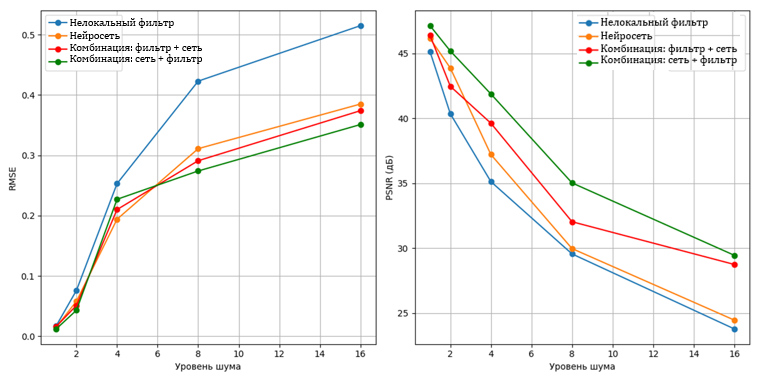
\includegraphics[keepaspectratio=true,scale=0.67] {my_folder/images/denoising/metrics_noise.png}
	\captionof{figure}{Визуальный анализ на синтетических данных для $\lambda=16$}
	\label{fig:synthetic-denoise-16}  
	\vspace{\mfloatsep} % интервал  	
\end{minipage}
\par Однако более информативными будут значения, приведённые в таблице \ref{tab:synthetic-denoise-16}. Из них можно сделать следующие выводы:
\begin{enumerate}
	\item Нелокальный фильтр (NLM) демонстрирует наименьшее время работы, но при этом имеет наибольшие значения RMSE и наименьшие значения PSNR среди всех рассмотренных методов.
	\item Нейросеть (N2N) требует больше времени на обработку, но достигает лучших результатов по сравнению с нелокальным фильтром как по RMSE, так и по PSNR.
	\item Комбинированные методы (фильтр+сеть и сеть+фильтр) показывают лучшие показатели по метрикам RMSE и PSNR в сравнении с нейросетевым подходом. При этом комбинация "сеть+фильтр" демонстрирует наилучшие результаты, чем "фильтр+сеть", как и в случае визуального анализа.
\end{enumerate}  
\begin{table} [H]% Пример оформления таблицы
	\centering\small
	\caption{Численный анализ на синтетических данных для $\lambda=16$}%
	\label{tab:synthetic-denoise-16}
	\begin{tabular}{|l|l|l|l|}
		\hline
		Методы&Время работы, с&RMSE&PSNR, дБ\\
		\hline
		Нелокальный фильтр, NLM
		&15&0.51&23.8\\ \hline
		Нейросеть, N2N&72&0.38&24.5\\ \hline
		Комбинация фильтр+сеть
		&87&0.37&28.7\\ \hline Комбинация сеть+фильтр
		&88&0.35&29.5\\ \hline		
	\end{tabular}
	\normalsize% возвращаем шрифт к нормальному
\end{table}
\par Также был проведён анализ работы методов в зависимости от уровня шума $\lambda \in [1, 2, 4, 8, 16]$. На \firef{fig:synthetic-denoise-16-all} можно увидеть, что лучшими по обоим показателям оказались комбинированные методы, а также что с увеличением уровня шума RMSE всех методов увеличивается, а PSNR соответственно уменьшается. Наименьшие значения RMSE и наибольшие значения PSNR достигаются при комбинации методов "сеть+фильтр", что свидетельствует о большей устойчивости этого подхода к высоким уровням шума.
\begin{minipage}{\textwidth}
	\centering
	\vspace{\mfloatsep} % интервал  	
	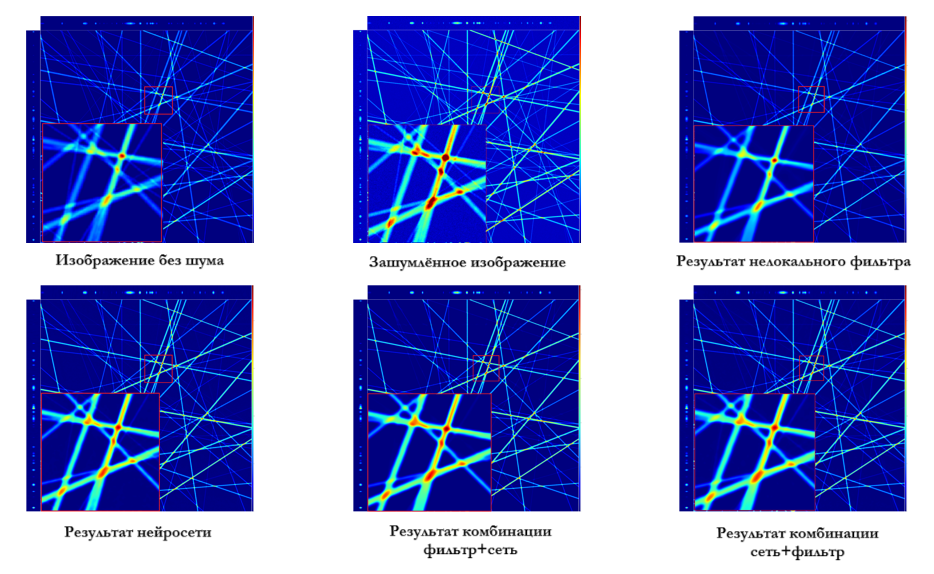
\includegraphics[keepaspectratio=true,scale=0.67] {my_folder/images/denoising/test_16_all.png}
	\captionof{figure}{Численный анализ на синтетических данных в зависимости от уровня шума $\lambda$}
	\label{fig:synthetic-denoise-16-all}  
	\vspace{\mfloatsep} % интервал  	
\end{minipage}
\par Таким образом, комбинированные подходы обеспечивают наилучшее качество денойзинга, несмотря на большее время обработки, что делает их предпочтительными для задач, где качество результата критично.
\subsubsection{Денойзинг реальных данных}
\par Для проверки работоспособности методов были проведены эксперименты по денойзингу на реальных данных. В этих экспериментах не будут представлены результаты метрик PSNR и RMSE, так как отсутствует точное изображение, с которым можно было бы сравнить обработанные данные.
\par  Помимо этого, был проведен анализ сегмента реального изображения, на котором отсутствует объект. Этот анализ включает вычисление основных статистических характеристик распределения, таких как среднее, дисперсия и среднеквадратическое отклонение (СКО). Проведение статистического анализа для области, содержащей фон, необходимо по нескольким причинам:
\begin{itemize}[]
	\item Оценка работоспособности методов денойзинга по удалению шумов на реальных снимках.
	\item Исследование природы шума и подтверждение его распределения по Пуассону.
\end{itemize}
\par Начнём с эксперимента на изображении трубочек размером 40x200x200. На \firef{fig:real-segment} приведены результаты денойзинга. На основании данных результатов можно сделать следующие выводы:
\begin{enumerate}[]
	\item Нелокальный фильтр справляется хорошо с шумами низкой интенсивности, однако сам объект остался в зашумлённом состоянии.
	\item Нейросеть успешно обесшумила весь снимок, сделав объект более чётким и очерченным.
	\item Комбинированные методы совместили достоинства обоих подходов. Интенсивности шумов на фоне изображения (где нет объекта) значительно уменьшились, что свидетельствует о высокой эффективности методов в удалении шумов. При этом комбинация "сеть + фильтр" лучше сглаживает шумы и сохраняет детали объекта по сравнению с комбинацией "фильтр + сеть".
\end{enumerate}
\par Также были посчитаны основные случайные величины в фоновом сегменте на данном снимке. Из полученных результатов в таблице  \ref{tab:real-segment} можно сделать следующие выводы:
\begin{enumerate}[]
	\item Добавочный шум на реальных снимках распределён по Пуассону, так как среднее и дисперсия практически  равны ($M[x] \approx D[x] = \lambda$, где $\lambda$ - возможный уровень шума)
	\item Нелокальный фильтр и нейросеть справляются с задачей, так как все измеряемые статистические величины уменьшаются.
	\item Комбинированные методы показывают улучшенные результаты: среднее значение интенсивности шума уменьшается более чем в 2 раза, а дисперсия уменьшается в 1.5 раза.
\end{enumerate}
\begin{minipage}{\textwidth}
	\centering
	\vspace{\mfloatsep} % интервал  	
	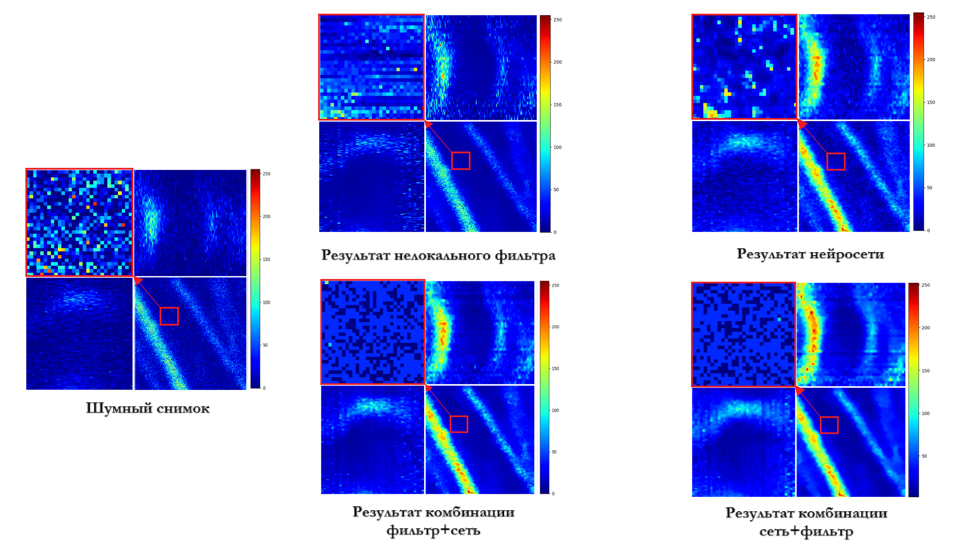
\includegraphics[keepaspectratio=true,scale=0.67] {my_folder/images/denoising/real_colors.png}
	\captionof{figure}{Денойзинг реального снимка; Сегмент, не содержащий объекта}
	\label{fig:real-segment}  
	\vspace{\mfloatsep} % интервал  	
\end{minipage}
\begin{table} [H]% Пример оформления таблицы
	\centering\small
	\caption{Статистика интенсивности шума на реальном снимке}%
	\label{tab:real-segment}		
	\begin{tabular}{|l|l|l|l|}
		\hline
		Методы&Среднее&Дисперсия&СКО\\
		\hline	
		Шумный снимок
		&8.3&8.4&2.9\\ \hline
		Нелокальный фильтр, NLM
		&6&3.1&1.6\\ \hline
		Нейросеть, N2N&5.5&3.3&1.8\\ \hline
		Фильтр+сеть
		&2.3&2.7&1.6\\ \hline Сеть+фильтр
		&2.2&2.8&1.7\\ \hline			
	\end{tabular}
	\normalsize% возвращаем шрифт к нормальному
\end{table}
\par Также для реальных снимков разных размеров были построены графики интенсивностей вдоль линии, отмеченной красной линией. На основе \firef{fig:intensity-test1-a} и табл. \ref{tab:intensity-test1} можно сказать, что:
\begin{enumerate}[]
	\item Время работы нелокального фильтра и нейросети практически не отличается из-за небольшого размера изображения.
	\item Нейросеть лучше подавляет пики интенсивностей, чем нелокальный фильтр.
	\item Комбинация "сеть+фильтр" даёт наиболее гладкий график интенсивностей, что указывает на более эффективное устранение шумов и сохранение деталей.
\end{enumerate}
\begin{figure}[H]
	\adjustbox{minipage=1.3em,valign=t}{\subcaption{}\label{fig:intensity-test1-a}}%
	\begin{subfigure}[t]{0.6\textwidth\relax}
		\centering
		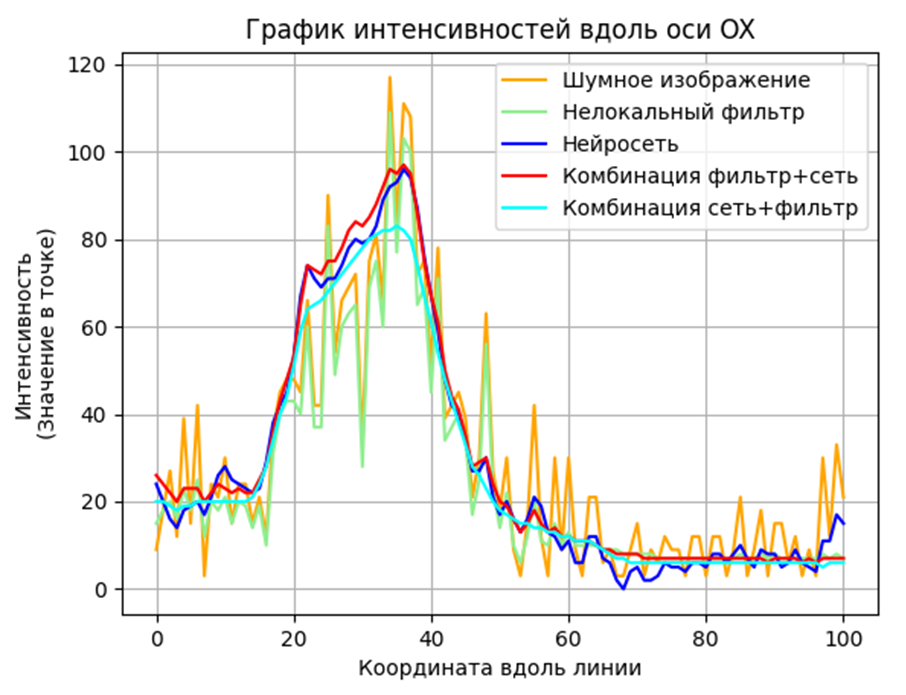
\includegraphics[width=.95\linewidth,valign=t]{my_folder/images/denoising/intensity_test1.png}
	\end{subfigure}
	\hfill %выровнять по ширине
	\adjustbox{minipage=1.3em,valign=t}{\subcaption{}\label{fig:denoise-train-b}}%
	\begin{subfigure}[t]{0.3\textwidth\relax}
		\centering
		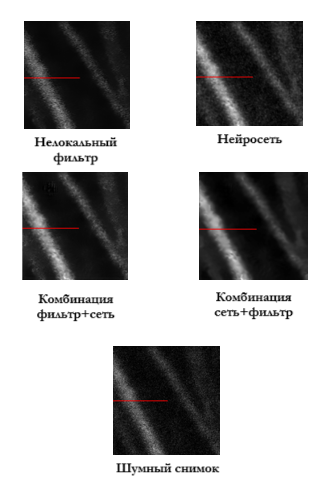
\includegraphics[width=.95\linewidth,valign=t]{my_folder/images/denoising/intensity_test1_images.png}
	\end{subfigure}
	\\[20pt]
	\captionsetup{justification=centering} %центрировать
	\caption{График интенсивностей вдоль оси OX для реального изображения размером 40x200x200: {\itshape a} --- График интенсивностей вдоль оси OX; {\itshape b} --- Результаты денойзинга} 
	\label{fig:intensity-test1}
\end{figure}
\begin{table} [H]% Пример оформления таблицы
	\centering\small
	\caption{Статистика интенсивности шума на реальном снимке}%
	\label{tab:intensity-test1}		
	\begin{tabular}{|l|l|l|l|l|}
		\hline
		 &Нелокальный фильтр&Нейросеть&Фильтр+сеть&Сеть+фильтр\\
		\hline	
		Время, cек.
		&1.5&1.5&3.1&3.2\\ \hline
	\end{tabular}
	\normalsize% возвращаем шрифт к нормальному
\end{table}
\par Для снимка большой размерности (29x2048x2048) были также применены различные методы денойзинга. Аналогично, для наглядности, построен график интенсивностей \firef{fig:intensity-test2-a}, проходящий сквозь объект снимка. Также было замерено время и записано в \ref{tab:intensity-test2}. Итак, можно заметить следующее: 
\begin{enumerate}[]
	\item  Нелокальный фильтр (NLM) работает значительно быстрее, чем нейросеть и комбинированные методы, но результат денойзинга значительно хуже.
	\item Нейросеть работает дольше, но даёт график интенсивностей с меньшим числом перепадов интенсивностей.
	\item График интенсивностей комбинированных методов показывает, что комбинации дают более гладкий результат, чем отдельно взятые методы, что свидетельствует о лучшем сохранении деталей и снижении шумов.
	\item Из двух комбинаций метод сеть+фильтр дает наиболее гладкий график интенсивностей и лучше сохраняет детали изображения.
\end{enumerate}
\begin{figure}[H]
	\adjustbox{minipage=1.3em,valign=t}{\subcaption{}\label{fig:intensity-test2-a}}%
	\begin{subfigure}[t]{0.6\textwidth\relax}
		\centering
		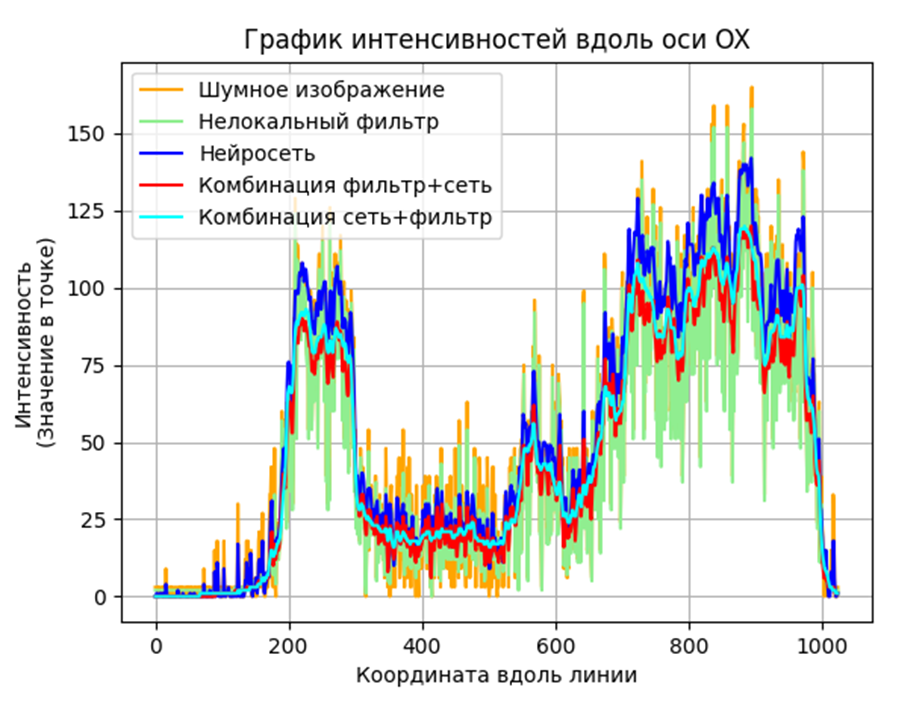
\includegraphics[width=.95\linewidth,valign=t]{my_folder/images/denoising/intensity_test2.png}
	\end{subfigure}
	\hfill %выровнять по ширине
	\adjustbox{minipage=1.3em,valign=t}{\subcaption{}\label{fig:intensity-test2-b}}%
	\begin{subfigure}[t]{0.3\textwidth\relax}
		\centering
		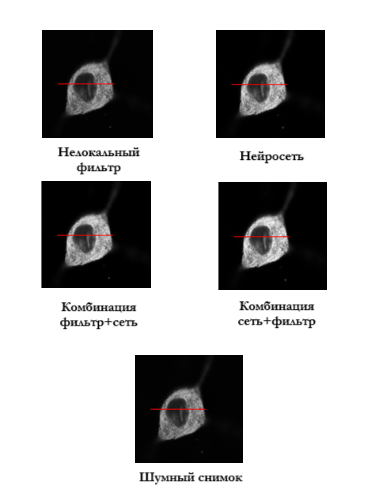
\includegraphics[width=.95\linewidth,valign=t]{my_folder/images/denoising/intensity_test2_images.png}
	\end{subfigure}
	\\[20pt]
	\captionsetup{justification=centering} %центрировать
	\caption{График интенсивностей вдоль оси OX для реального изображения размером 29x2048x2048: {\itshape a} --- График интенсивностей вдоль оси OX; {\itshape b} --- Результаты денойзинга} 
	\label{fig:intensity-test2}
\end{figure}
\begin{table} [H]% Пример оформления таблицы
	\centering\small
	\caption{Статистика интенсивности шума на реальном снимке}%
	\label{tab:intensity-test2}		
	\begin{tabular}{|l|l|l|l|l|}
		\hline
		&Нелокальный фильтр&Нейросеть&Фильтр+сеть&Сеть+фильтр\\
		\hline	
		Время
		&51 сек.&4.6 мин.&5.1 мин.&5.2 мин.\\ \hline
	\end{tabular}
	\normalsize% возвращаем шрифт к нормальному
\end{table}

\section{Результаты автоматической сегментации}
\par Результаты показывают, что алгоритм автоматической сегментации сфер имеет значительное преимущество перед ручной сегментацией. На примере изображения размером \textbf{36x2048x2048} время выполнения для автосегментации составило всего \textbf{0.83 секунды} с усреднением и 0.78 секунды без усреднения, в то время как \textbf{ручная сегментация} занимает значительно больше времени, около \textbf{10-15 минут}. Эксперименты для 2-ух сегментаций проводились на CPU: \textbf{AMD Ryzen 7 5700U with Radeon Graphics 1.80 GHz}.

\par На \firef{fig:autosegm-res} приведено визуальное представление результата автосегментации:\\
\noindent % for correct centering
\begin{minipage}{\textwidth}
	\centering
	\vspace{\mfloatsep} % интервал  	
	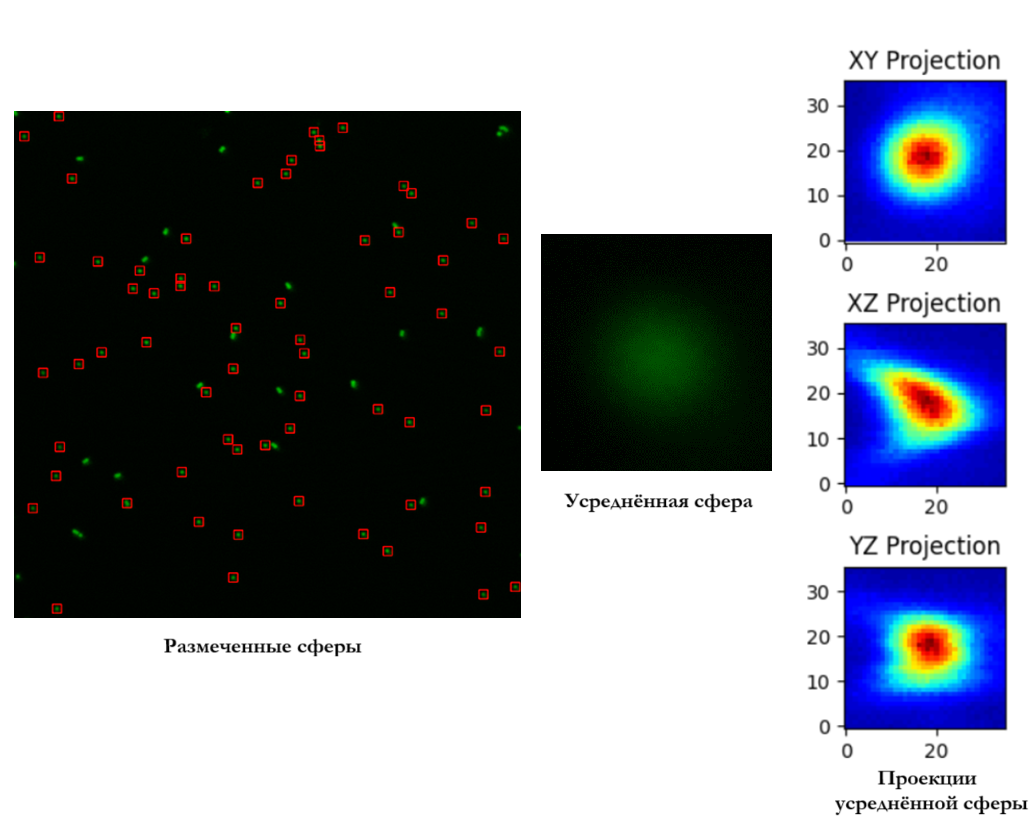
\includegraphics[keepaspectratio=true,scale=0.37] {my_folder/images/autosegm/autosegm_res.png}
	\captionof{figure}{Результат автоматической сегментации сфер}\label{fig:autosegm-res}  
	\vspace{\mfloatsep} % интервал  	
\end{minipage}

\par Применение денойзинга значительно улучшает качество изображений.  На \firef{fig:autosegm-res-denoise} можно увидеть, что предварительно обработанное изображение со сферами нейронной сетью Noise2Noise, после процесса сегментации и усреднения даёт более округлую и отчётливую усреднённую сферу. 
\begin{minipage}{\textwidth}
	\centering
	\vspace{\mfloatsep} % интервал  	
	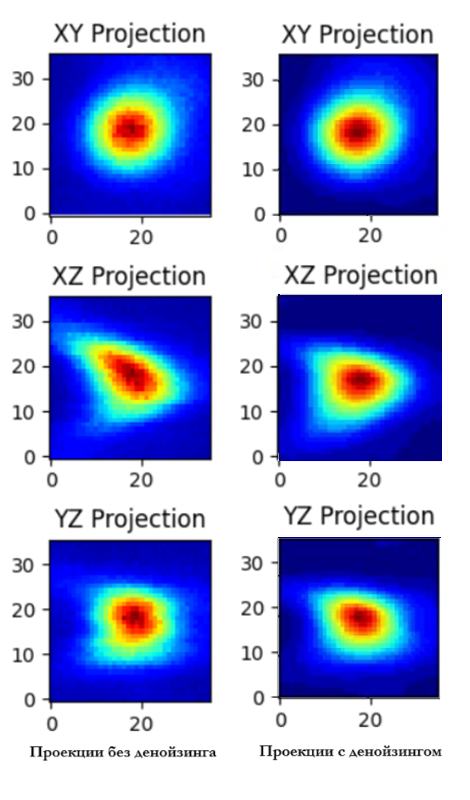
\includegraphics[keepaspectratio=true,scale=0.57] {my_folder/images/autosegm/autosegm_res_denoised.png}
	\captionof{figure}{Сравнение результатов сегментации сфер с и без денойзинга}\label{fig:autosegm-res-denoise}  
	\vspace{\mfloatsep} % интервал  	
\end{minipage}

\par Всё выше перечисленное говорит о том, что использование автоматической сегментации сфер оправдано, особенно учитывая сложность и время, затрачиваемое на ручную сегментацию при большом количестве сфер на изображении. Применение предварительного денойзинга дополнительно улучшает точность и качество сегментации, что делает этот подход еще более полезным для обработки изображений с высоким уровнем шума. 

\section{Описание архитектуры онлайн-сервиса деконволюции}
\par Результат проделанной работы был оформлен в виде онлайн-сервиса с встроенными процессами обработки изображений с помощью языков программирования Python и JavaScript. Архитектура сервиса включает следующие технологии и инструменты: Django, ReactJS, Docker, Redis, Nginx, Celery, Flower.
\par Все процессы улучшения изображений могут быть представлены в виде идущими друг за другом шагами обработки: например, загрузка изображений, настройка параметров, обработка, сохранение и визуализация результатов. Потому веб-интерфейс каждой отдельной функциональности представляемого ПО реализован в виде степпера (от англ. step - шаги). Данный степпер даёт возможность пользователю наблюдать  промежуточные результаты на каждом шаге обработки данных, а также на этапах до и после обработки. Кроме того в переходах между разными этапами (степперами) результаты на предыдущем шаге сохраняются в кэше (высокоскоростной памяти небольшого размера), чтобы минимизировать задержки при доступе к данным. 
\par Архитектура серверной части поддерживает масштабируемость, гибкость, высокую производительность, мониторинг и логгирование, а также сервис является надёжным и простым в использовании благодаря контейнеризации Docker. Также сервис обладает модульностью - возможностью интеграции с ПО лаборатории и загрузки изображений в базу данных (БД).
\par Итак, перейдём к рассмотрению конкретных этапов обработки изображений:
\begin{enumerate}[]
	\item \textit{Сегментация (извлечение) флуоресцентных сфер}:\\
	На данном этапе (см. \firef{fig:bead-stepper}) пользователь может гибко комбинировать два подхода к сегментации: ручной и автоматический. Настройка параметров и использование слайдеров значительно упрощает процесс извлечения образцов для пользователя.\\
	\begin{minipage}{\textwidth}
		\centering
		\vspace{\mfloatsep} % интервал  	
		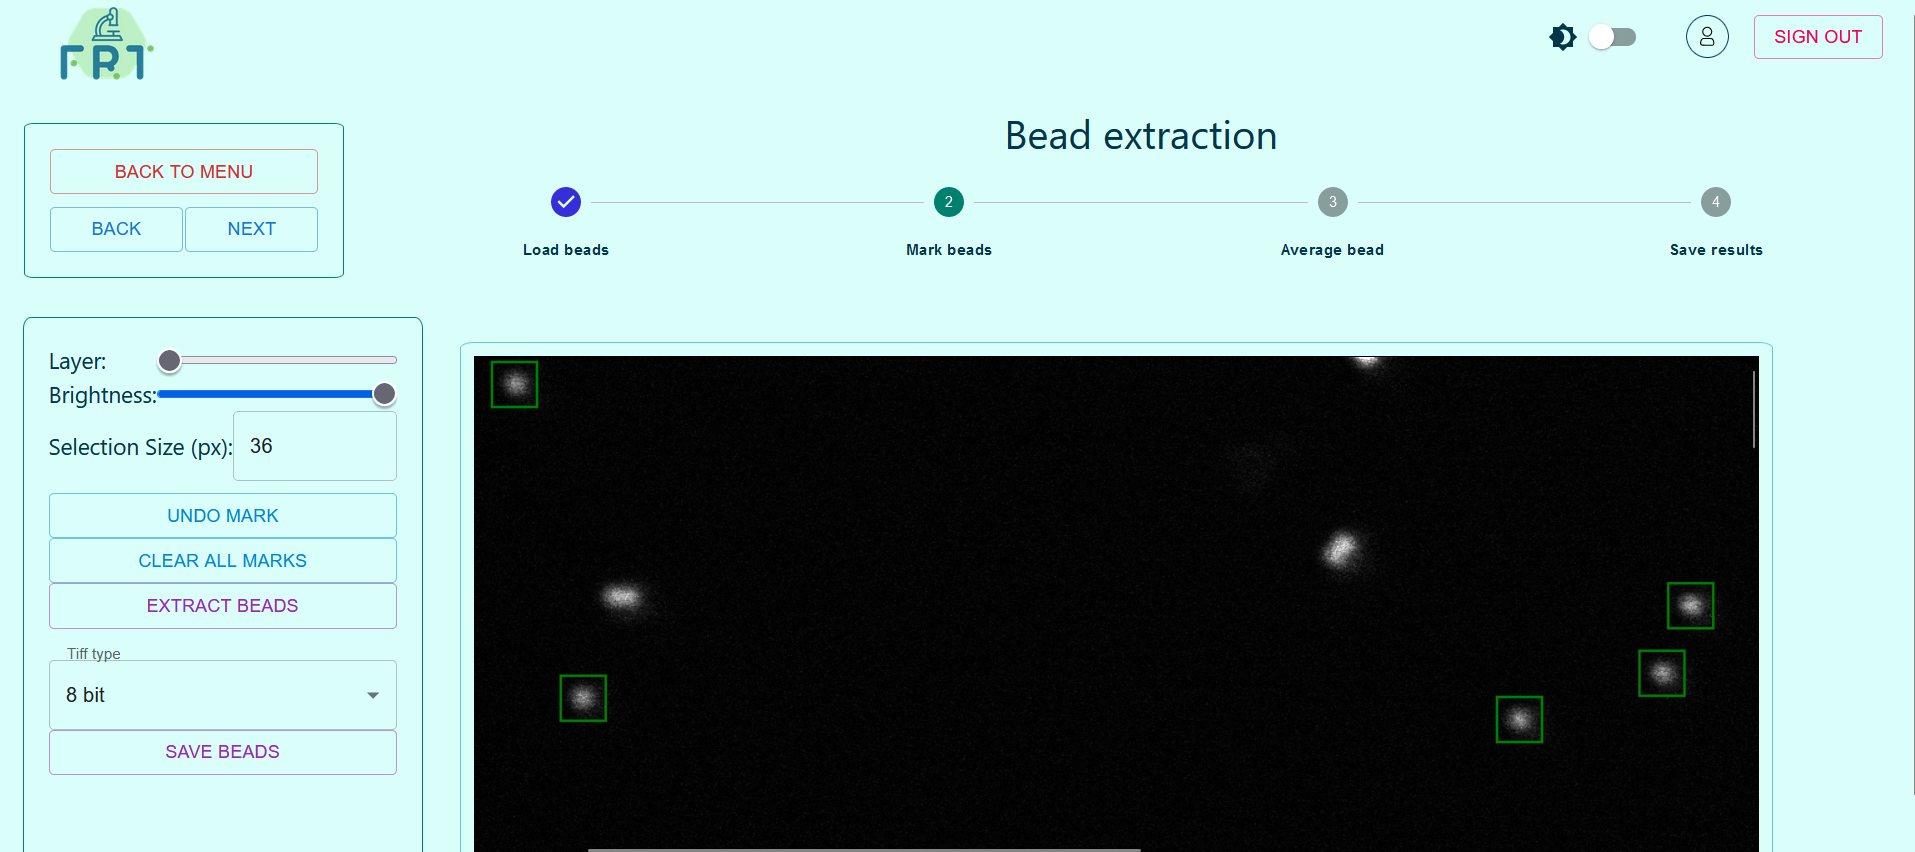
\includegraphics[keepaspectratio=true,scale=0.25] {my_folder/images/online_service/steper_extractor.png}
		\captionof{figure}{Процесс сегментации сфер}\label{fig:bead-stepper}  
		\vspace{\mfloatsep} % интервал  	
	\end{minipage}
\item \textit{Усреднение сфер}:\\
На данном этапе (см. \firef{fig:avg-stepper}) есть возможность просмотра выбранных сфер, их усреднение с выбором метода предобработки.\\
\begin{minipage}{\textwidth}
	\centering
	\vspace{\mfloatsep} % интервал  	
	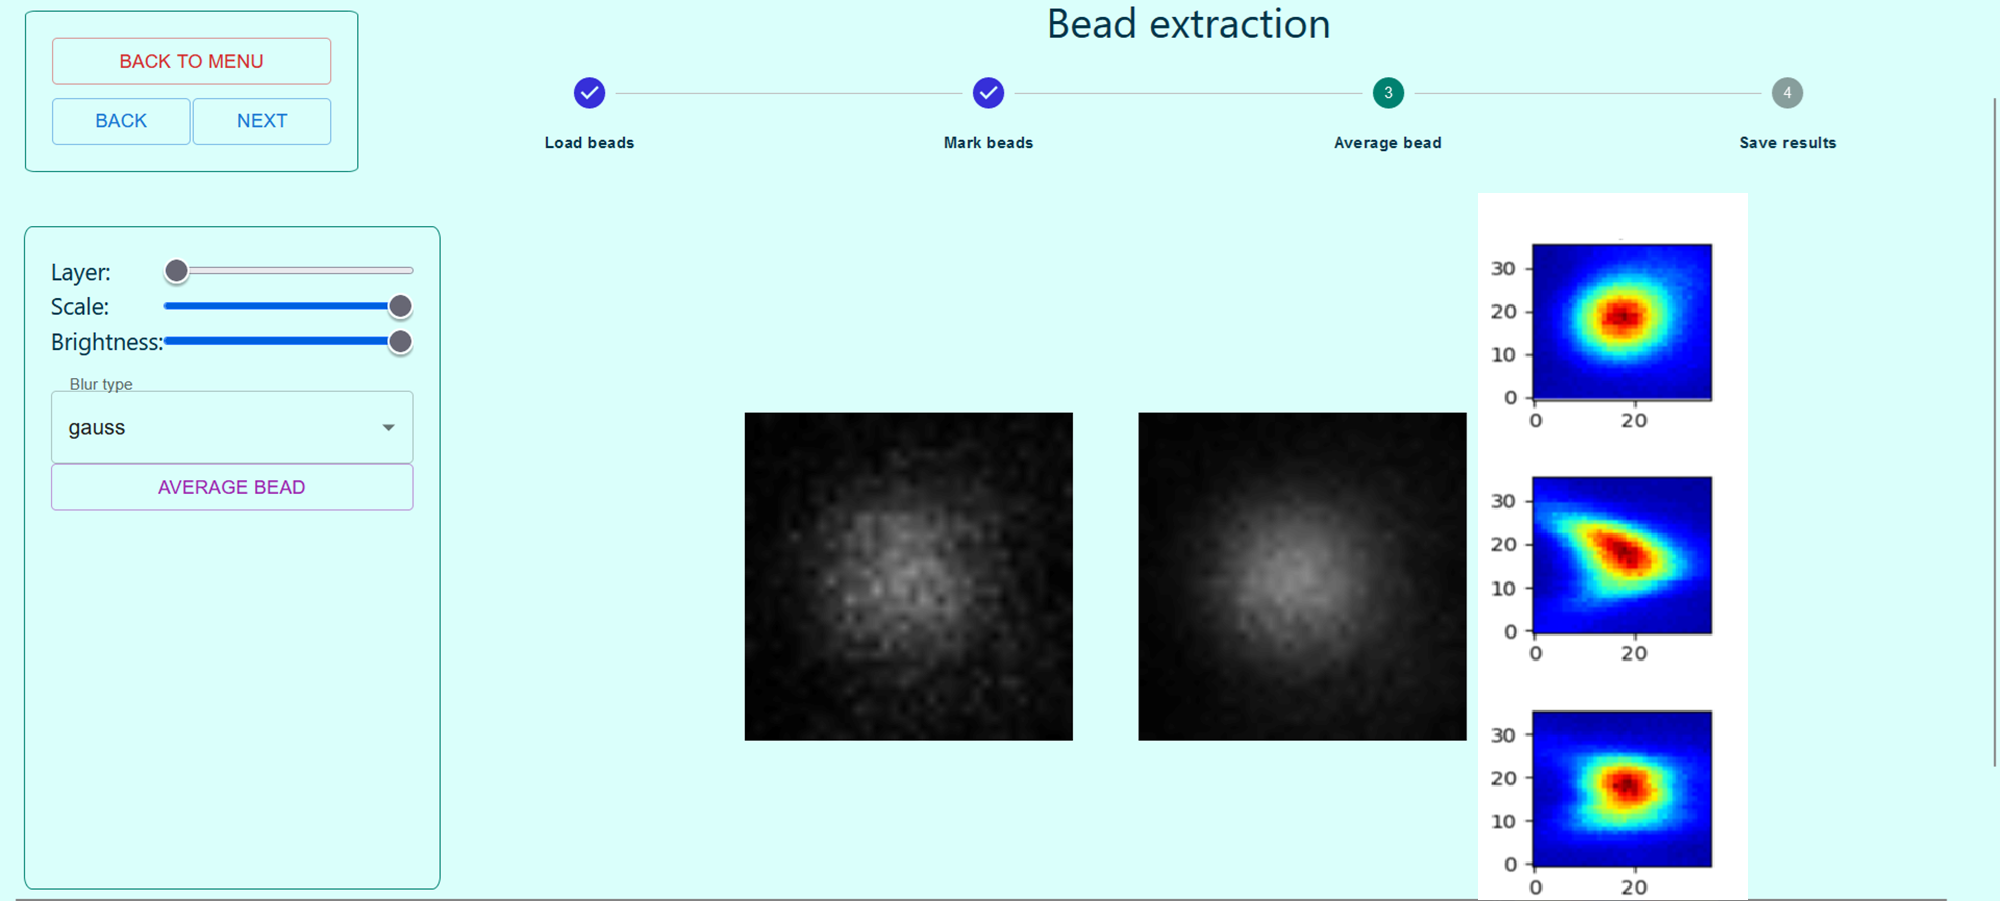
\includegraphics[keepaspectratio=true,scale=0.25] {my_folder/images/online_service/averaging_bead.png}
	\captionof{figure}{Процесс усреднения трёхмерных сфер}\label{fig:avg-stepper}  
	\vspace{\mfloatsep} % интервал  	
\end{minipage}
\item \textit{Вычисление Функции рассеяния точки (ФРТ)}:\\
На 2-ой степпер (см. \firef{fig:psf-stepper}) предзагружается усреднённая сфера и пользователь можеть получить ФРТ эксперементальным способом, применяя метод деконволюции, меняя различные гиперпараметры: размер сферы, число иттераций, параметр регуляризации и вид метода Ричардсона-Люси (РЛ).\\
\begin{minipage}{\textwidth}
	\centering
	\vspace{\mfloatsep} % интервал  	
	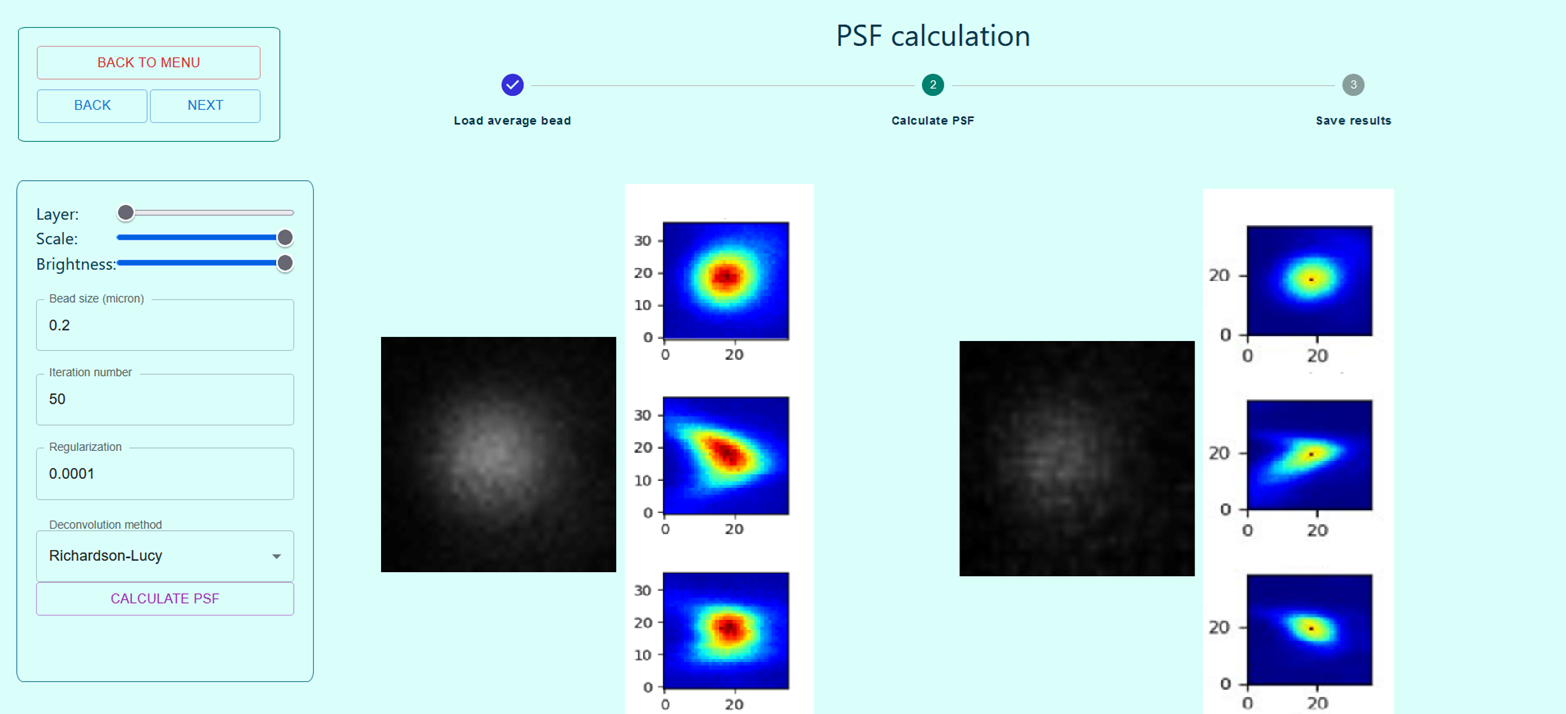
\includegraphics[keepaspectratio=true,scale=0.3] {my_folder/images/online_service/stepper_psf.png}
	\captionof{figure}{Процесс вычисления ФРТ}\label{fig:psf-stepper}  
	\vspace{\mfloatsep} % интервал  	
\end{minipage}
\item \textit{Деконволюция трёхмерного изображения}:\\
В последнем степпере (см. ) загружается эФРТ и в интерактивном формате, аналогично вычислению ФРТ, пользователь может обработать трёхмерное изображение в реальном времени. Как можно увидеть на \firef{fig:deconv-stepper}, что результат деконволюции сделал сферы более отчётливыми и отделимыми друг от друга. \\
\begin{minipage}{\textwidth}
	\centering
	\vspace{\mfloatsep} % интервал  	
	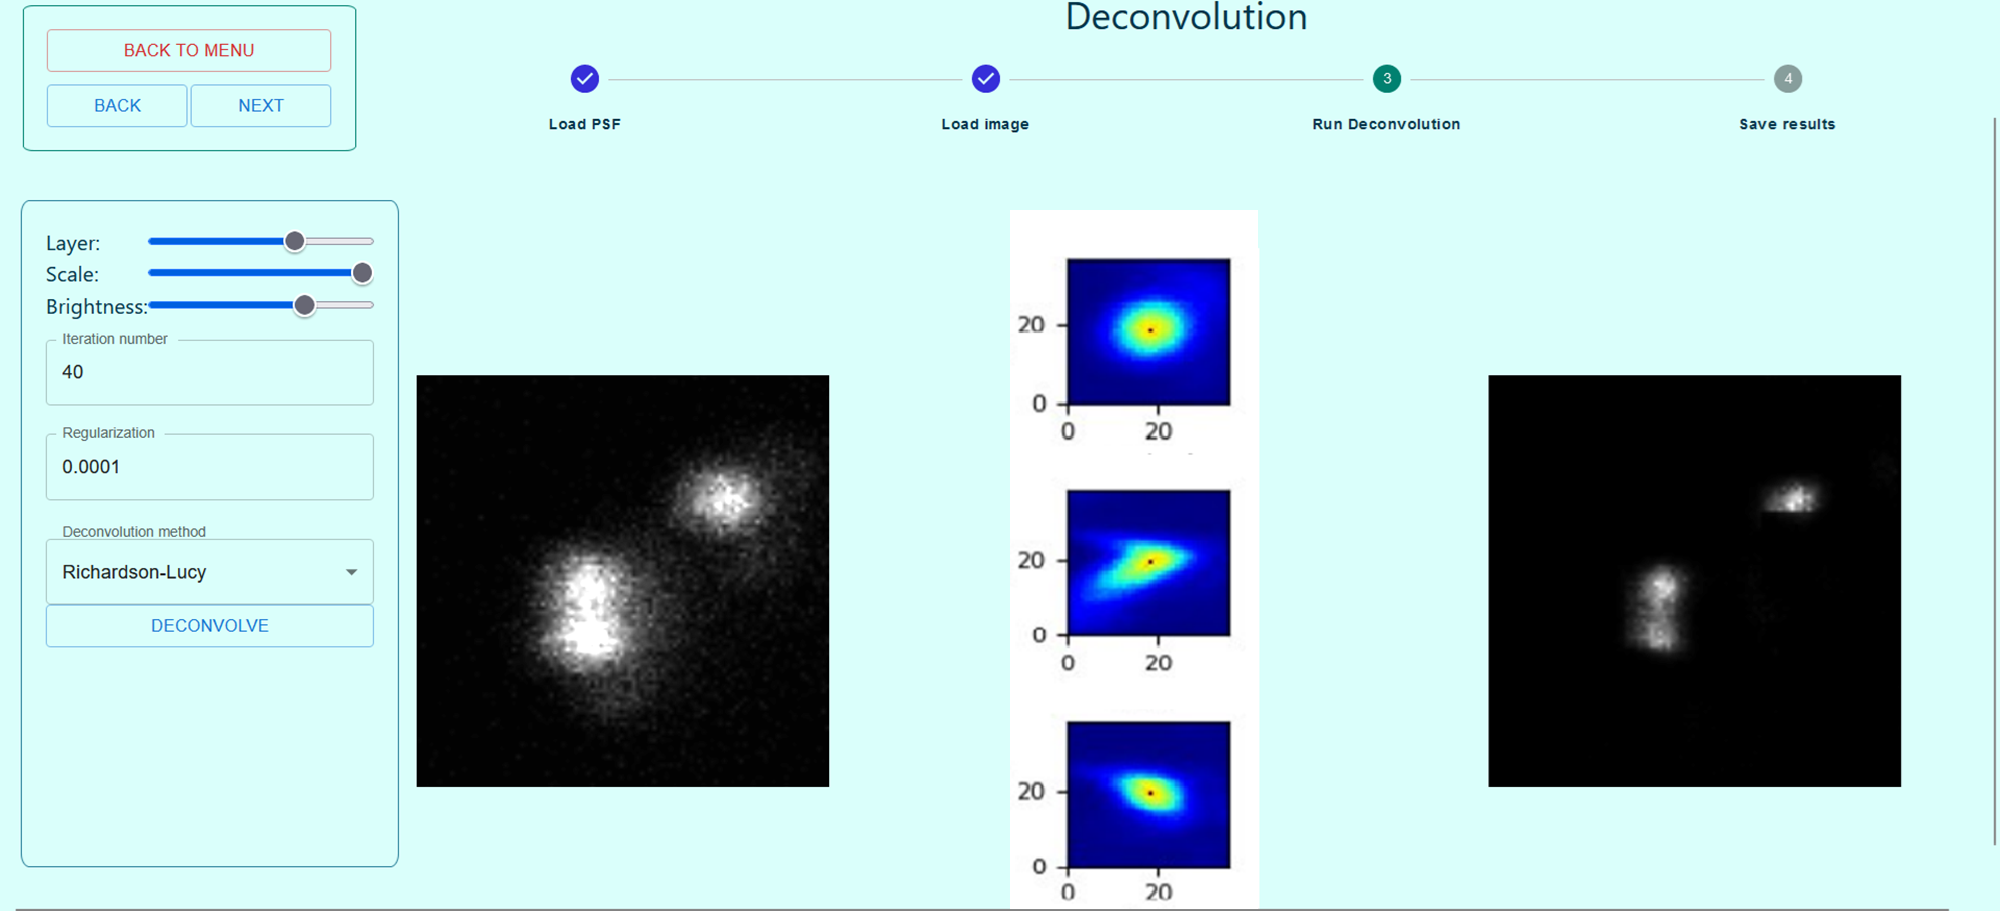
\includegraphics[keepaspectratio=true,scale=0.25] {my_folder/images/online_service/deconvolution.png}
	\captionof{figure}{Процесс деконволюции изображений}\label{fig:deconv-stepper} 
	\vspace{\mfloatsep} % интервал  	
\end{minipage}
\end{enumerate}

% не рекомендуется использовать отдельную section <<введение>> после лета 2020 года
%\section{Введение} \label{ch3:intro}


%% Вспомогательные команды - Additional commands
%
%\newpage % принудительное начало с новой страницы, использовать только в конце раздела
%\clearpage % осуществляется пакетом <<placeins>> в пределах секций
%\newpage\leavevmode\thispagestyle{empty}\newpage % 100 % начало новой страницы           	 % Глава 3           	 % Глава 3
\ContinueChapterEnd % завершить размещение глав <<подряд>>
%% Завершение основной части

\chapter*{Заключение} \label{ch-conclusion}
\par В данной работе были рассмотрены существующие методы обесшумливания двухмереных изображений, такие как нелокальный фильтр среднего (Non-local means), а также метод глубокого обучения Noise2Noise. На основе изученного материала был разработан алгоритм 3D денойзинга, включающий в себя эти 2 подхода, а также комбинирующий их. На основе полученных результатов денойзинга можно сделать следующие выводы:
\begin{itemize}[]
	\item Нелокальный фильтр демонстрирует высокую скорость работы и эффективно удаляет шумы с низкой интенсивностью.
	\item Нейросетевой метод позволяет удалять шумы на всём изображении. Метрики качества, такие как PSNR и RMSE, превосходят показатели нелокального фильтра примерно  на 15\%.
	\item Комбинирование вышеупомянутых методов позволило добиться улучшения метрик PSNR и RMSE на 10\% по сравнению с нейросетевым подходом, а также обеспечивают наиболее гладкий график интенсивностей на выходе.
	\item Шум, наблюдаемый на реальных снимках приближен к распредению Пуассона.
	\item Результы методов на реальных снимках показывают уменьшение дисперсии шума, что также доказывает работоспобность методов шумоподавления.
	\item Комбинированные методы имеют меньшие значения средних и дисперсий, что также подтверждает улучшения качества работы при комбинации методов.
\end{itemize}
\par Также был разработан алгоритм автоматической сегментации флуоресцентных сфер, который позволил ускорить процесс ручной сегментации на 2 порядка.
\par Все разработнные алгоритмы были успешно интегрированы и развернуты в веб-сервисе, созданном в сотрудничестве с Лабораторией молекулярной нейродегенерации.         	 % Заключение

%% Наличие следующих перечней не исключает расшифровку сокращения и условного обозначения при первом упоминании в тексте!
\chapter*{Список сокращений и условных обозначений}             % Заголовок
\addcontentsline{toc}{chapter}{Список сокращений и условных обозначений}  % Добавляем его в оглавление
\noindent
\addtocounter{table}{-1}% Нужно откатить на единицу счетчик номеров таблиц, так как следующая таблица сделана для удобства представления информации по ГОСТ
%\begin{longtabu} to \dimexpr \textwidth-5\tabcolsep {r X}

\begin{tabular*}{\textwidth}{rl} % Таблицу не прорисовываем!
% Жирное начертание для математических символов может иметь
% дополнительный смысл, поэтому они приводятся как в тексте
% диссертации
\textbf{ФРТ} & Функция рассеяния точки. \\
\textbf{DOI} & Digital Object Identifier. \\
\textbf{WoS} & Web of Science. \\
\textbf{ВКР}  & Выпускная квалификационная работа. \\
\textbf{ТГ-объект}  & Текстово-графический объект. \\
%$\begin{rcases}
%a_n\\
%b_n
%\end{rcases}$  & 
%\begin{minipage}{\linewidth}
%Коэффициенты разложения Ми в дальнем поле, соответствующие
%электрическим и магнитным мультиполям.
%\end{minipage}
%\\
%${\boldsymbol{\hat{\mathrm e}}}$ & Единичный вектор. \\
%$E_0$ & Амплитуда падающего поля.\\
%$\begin{rcases}
%a_n\\
%b_n
%\end{rcases}$  & 
%Коэффициенты разложения Ми в дальнем поле соответствующие
%электрическим и магнитным мультиполям ещё раз, но без окружения
%minipage нет вертикального выравнивания по центру.
%\\
%$j$ & Тип функции Бесселя.\\
%$k$ & Волновой вектор падающей волны.\\
%
%$\begin{rcases}
%a_n\\
%b_n
%\end{rcases}$  & 
%\begin{minipage}{\linewidth}
%\vspace{0.7em}
%Коэффициенты разложения Ми в дальнем поле соответствующие
%электрическим и магнитным мультиполям, теперь окружение minipage есть
%и добавленно много текста, так что описание группы условных
%обозначений значительно превысило высоту этой группы... Для отбивки
%пришлось добавить дополнительные отступы.
%\vspace{0.5em}
%\end{minipage}
%\\
%$L$ & Общее число слоёв.\\
%$l$ & Номер слоя внутри стратифицированной сферы.\\
%$\lambda$ & Длина волны электромагнитного излучения
%в вакууме.\\
%$n$ & Порядок мультиполя.\\
%$\begin{rcases}
%{\mathbf{N}}_{e1n}^{(j)}&{\mathbf{N}}_{o1n}^{(j)}\\
%{\mathbf{M}_{o1n}^{(j)}}&{\mathbf{M}_{e1n}^{(j)}}
%\end{rcases}$  & Сферические векторные гармоники.\\
%$\mu$  & Магнитная проницаемость в вакууме.\\
%$r,\theta,\phi$ & Полярные координаты.\\
%$\omega$ & Частота падающей волны.\\
%
%  \textbf{BEM} & Boundary element method, метод граничных элементов.\\
%  \textbf{CST MWS} & Computer Simulation Technology Microwave Studio.
\end{tabular*}
		         % Необязательная рубрика! Список сокращений и условных обозначений

\input{my_folder/dictionary}    		 % Необязательная рубрика! Словарь терминов
% По порядку после Списка сокращений и условных обозначений, если есть.	


%%% Не мянять - Do not modify
%%
%%
\clearpage                                  % В том числе гарантирует, что список литературы в оглавлении будет с правильным номером страницы
%\hypersetup{ urlcolor=black }               % Ссылки делаем чёрными
%\providecommand*{\BibDash}{}                % В стилях ugost2008 отключаем использование тире как разделителя 
\urlstyle{rm}                               % ссылки URL обычным шрифтом
\ifdefmacro{\microtypesetup}{\microtypesetup{protrusion=false}}{} % не рекомендуется применять пакет микротипографики к автоматически генерируемому списку литературы
%\newcommand{\fullbibtitle}{Список литературы} % (ГОСТ Р 7.0.11-2011, 4)
%\insertbibliofull  
%\noindent
%\begin{group}
\chapter*{Список использованных источников}	
\label{references}
\addcontentsline{toc}{chapter}{Список использованных источников}	% в оглавление 
\printbibliography[env=SSTfirst]                         % Подключаем Bib-базы
%\ifdefmacro{\microtypesetup}{\microtypesetup{protrusion=true}}{}
%\urlstyle{tt}                               % возвращаем установки шрифта ссылок URL
%\hypersetup{ urlcolor={urlcolor} }          % Восстанавливаем цвет ссылок



%\urlstyle{rm}                               % ссылки URL обычным шрифтом
%\ifdefmacro{\microtypesetup}{\microtypesetup{protrusion=false}}{} % не рекомендуется применять пакет микротипографики к автоматически генерируемому списку литературы
%\insertbibliofull                           % Подключаем Bib-базы
%\ifdefmacro{\microtypesetup}{\microtypesetup{protrusion=true}}{}
%\urlstyle{tt}                               % возвращаем установки шрифта ссылок URL		     % Список литературы

% Здесь можно поместить список иллюстративного материала

\appendix % не редактировать / keep unmodified


\input{my_folder/appendix1}			     % Приложение 1

\input{my_folder/appendix2}			 	 % Приложение 2


\end{document} % конец документа


%%% Удачной защиты ВКР! - Good luck on the thesis defense!
%%
%%% Поддержать проект
%%
%% Запросы на добавление / изменение просим писать на следующей странице:
%% https://github.com/ParkhomenkoV/SPbPU-student-thesis-template/issues
%%
%% Список пожеланий в файле шаблона <<TO-DO-list.tex>>
%%
%% Благодарности просим указывать в виде 
%%
%% 1. Добавление <<Звезды>> проекту https://github.com/ParkhomenkoV/SPbPU-student-thesis-template/stargazers
%%
%% 2. Добавления <<Сердечка>> и репоста проекта в социальных сетях:
%%		https://vk.com/latex_polytech 
%%		https://www.fb.com/groups/latex.polytech
%%

%%% Support project
%%
%% Requests on adding / modifications is better to be publishen on the following web-page:
%% https://github.com/ParkhomenkoV/SPbPU-student-thesis-template/issues
%%
%% Wishlist is in the template's file called <<TO-DO-list.tex>>
%%
%% Acknowledgements are better to be done in the form of 
%%
%% 1. Adding <<Star>> to the project https://github.com/ParkhomenkoV/SPbPU-student-thesis-template/stargazers
%%
%% 2. Adding <<Likes>> and Project repost in the social networks:
%%		https://vk.com/latex_polytech 
%%		https://www.fb.com/groups/latex.polytech
%% 

% Check list при передаче ВКР:
% - Количество страниц в Задании 2. Если нет, то комментирование последней строки в my_task.tex
% - Зачистка всех вспомогательных файлов (Clear auxilary files) и компиляция ВКР не менее 3х раз